% Inbuilt themes in beamer
\documentclass{beamer}


%Defining some colours
\definecolor{darkred}{rgb}{0.8,0,0}

% Theme choice: there a number of preset themes to choose from
% Play around with them, Cambridge is nice for first pres
%\usetheme{Szeged}
\usetheme{CambridgeUS} %setting the main theme
\usecolortheme{whale} % setting colour theme
\usefonttheme{professionalfonts} %font theme
\useinnertheme[shadow=true]{rounded}
%\useoutertheme{} %outer theme

%\setbeamertemplate{footline} %Remove footer line in all slides
\setbeamertemplate{navigation symbols}{} %removes navigation symbols
\setbeamertemplate{footline}[page number] %removes footer line, keeps pg#
\setbeamertemplate{caption}{\insertcaption} 


%Setting colours for boxes and captions
\setbeamercolor{block title}{bg=blue!30, fg=black}
\setbeamercolor{block body}{bg=blue!10}
\setbeamercolor{frametitle}{fg=black}

%%%FOR VIDEOS
\usepackage{media9}
\usepackage{multimedia}
% For the Flowchart
%\usepackage{tikz}
%\usetikzlibrary{shapes.geometric, arrows}
%\tikzstyle{startstop} = [rectangle, rounded corners, minimum width=3cm, minimum height=1cm,text centered, draw=black, fill=blue!30]
%\tikzstyle{process} = [rectangle, minimum width=3cm, minimum height=1cm, text centered, draw=black, fill=orange!30]
%\tikzstyle{decision} = [diamond, minimum width=3cm, minimum height=1cm, text centered, draw=black, fill=green!30]
%\tikzstyle{arrow} = [thick,->,>=stealth]

%%% For the Timeline
\usepackage{xcolor}
\usepackage{tikz} \usetikzlibrary{calc, arrows.meta, intersections, patterns, positioning, shapes.misc, fadings, through,decorations.pathreplacing}

\definecolor{ColorOne}{rgb}{0.0,0.5,1.0} %Lightblue
\definecolor{ColorTwo}{rgb}{1.0,0.6,0.4} %lightorange
\definecolor{ColorThree}{rgb}{0.75,0.58,0.89} %lightpurple

% Title page details: 
\title[BEAP Dec 2022]{Cells at War: The Playfulness of Game-Based Learning} 
\author{Alexander Turco}
\date{December 5, 2022}
\logo{
\includegraphics[height=1cm, width=1cm]{logo.png}}

% Bibliography stuff
\usepackage[natbib=true, sorting=nyt, style=authoryear-comp]{biblatex}
\addbibresource{ABC1.bib}

%Extra packages
\usepackage{makecell}

%For itemize
\setbeamertemplate{itemize item}[triangle]



\begin{document}
	
	% For my introduction slides, there will be the slide with my title and name as well as an outline slide with the brief overview of what I will discuss.
	% Title page frame - SLIDE 1%%%%%%%%%%%%%%%%%%%%%%%%%%%%%%%%%%%%%%%%%%%%%%%%%%%%%%%%%%%%%%%%%%%%%%%%%%%%%%%%%%%%%%%%%%%%%%%%%%%%%%%%%%%%%%%%%%%%%%%%%%%%%%%%%%%%
	\section{Introduction}
	\begin{frame}
		\titlepage 
		\begin{center}
			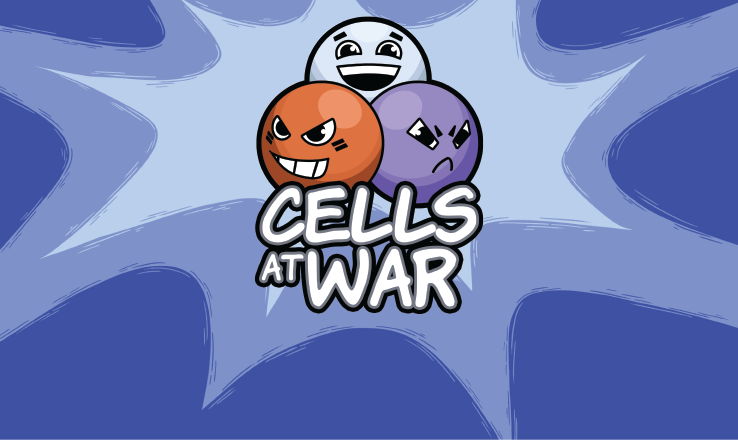
\includegraphics[width=7cm, height=4cm]{cellsatwar.png}
		\end{center}
	\end{frame}
	
	% Remove logo from the next slides
	\logo{}
	
	% Outline frame - SLIDE 2
	\begin{frame}{Overview}
		
		\begin{center}
		\begin{minipage}{6cm}
				
		  		\begin{block}{} \hyperlink{link1}{Background Information} \end{block}
		  		\begin{block}{} The Game Design Process \end{block}
		  		\begin{block}{} Collection of Student Feedback \end{block}
		  		\begin{block}{} Results \end{block}
		  		\begin{block}{} Conclusions \end{block}
		  		\begin{block}{} Future Work \end{block}

		\end{minipage}
		\end{center}
	
	\end{frame}
	
	% For my Background slides, I will talk about important things such as WHat LCRs are, their evolution, stuff like that
	% SLIDE 3 - WHAT ARE LCRs%%%%%%%%%%%%%%%%%%%%%%%%%%%%%%%%%%%%%%%%%%%%%%%%%%%%%%%%%%%%%%%%%%%%%%%%%%%%%%%%%%%%%%%%%%%%%%%%%%%%%%%%%%%%%%%%%%%%%%%%%%%%%%%%%%%%%%
	% The graphic for this slide is an image of some output from segA with the parameters in the brackets
	\section{Background}
	\begin{frame}{What is Game-based Learning?}
		\label{link1}
		
		\begin{itemize}
			\item Utilizing games in educational settings as an interactive medium to promote {\color{blue}\textbf{higher-order thinking}}, {\color{blue}\textbf{social skills}}, and {\color{blue}\textbf{problem-solving skills}} \newline
			\item Games support learning through {\color{blue}\textbf{engagement}}, {\color{blue}\textbf{motivation}}, {\color{blue}\textbf{interactivity}}, 
			{\color{blue}\textbf{drill and practice}}, and {\color{blue}\textbf{content mastery}} \newline
			\item In the digital era, game-based learning commonly refers to the use of {\color{blue}\textbf{digital games}} as effective instructional tools which also help develop {\color{blue}\textbf{digital proficiency}} 
			
			\footnotetext[1]{\tiny\cite{brown1989situated, jan2016game}}
		\end{itemize}
		
	\end{frame}

	% SLIDE 4 - I do Not Know if I am including this slide
	% The Graphic for this slide is an  
	% Entropy, which is measured by Shannon's Entropy equation is a measure of compositional complexity which uses the proportion of residue(s)
	% in a subsequence to measure the compositional state of that subseequence - A lower variety of residues = lower entropy 
	%\begin{frame}{Shannon's Entropy - MAYBE }
		
	%		$H = -L\sum p_i log_2(p_i)$
		
	%\end{frame}

	%SLIDE 5 - LCR's PRESENT IN UNIQUE WAYS
	\begin{frame}{The Benefits of Playing Video Games}
		
		\begin{block}{\textit{Interactive}}
			 \begin{itemize}
			 \item Individuals respond to situations presented in games, allowing them to think critically and strategize
			 \end{itemize}
		\end{block} \pause
	
		\begin{block}{\textit{Stimulating}}
			\begin{itemize}
				\item Individuals become addicted to the hormone boost their brains receive when they achieve results
			\end{itemize}
		\end{block} \pause
	
		\begin{block}{\textit{Exploratory}}
			\begin{itemize}
				\item Individuals are immersed in a world without boundaries, free to explore in any way they wish
			\end{itemize}
		\end{block}
	
	\footnotetext[2]{\tiny\cite{coller2009effectiveness, tomavska2022let}}
	
	\end{frame}

	%SLIDE 6 Limitations of Implementing Game-Based Learning
	\begin{frame}{The Limitations of Implementing Game-based Learning}
		\begin{enumerate}
			\item Many individuals believe that playing video games in a class setting will serve to act only as a source of entertainment and amusement rather than for educative purposes \newline 
			\item Educators are rarely involved in the development of educational video games \newline
			\item Teachers lack the technological and pedagogical supports to develop their understanding of game-based learning in the classroom 
			
		\end{enumerate}
	
	\footnotetext[3]{\tiny\cite{lister2015gamification,mayer2010adding,molin2017role,fishman2014empowering}}
		
	\end{frame}

	%%%%% APPRACH SECTION BEGINS HERE, 2 SLIDES
	\section{Approach}
	
	\begin{frame}{Cells at War Game Design Process}
		\tikzstyle{descript} = [text = black,align=center, minimum height=1.8cm, align=center, outer sep=0pt,font = \footnotesize]
		\tikzstyle{activity} =[align=center,outer sep=1pt]
		
		\begin{tikzpicture}[very thick, black]
			\small
			
			%% Coordinates
			\coordinate (O) at (-0.25,0); % Origin
			\coordinate (P1) at (4,0);
			\coordinate (CD) at (3,0);
			\coordinate (GP) at (9,0);
			\coordinate (P2) at (8,0);
			\coordinate (P3) at (11,0);
			\coordinate (E1) at (10,0);
			\coordinate (D1) at (1.7,0);
			\coordinate (F) at (11.5,0); %End
			
			%% Filled regions
			\fill[color=ColorOne!20] rectangle (O) -- (CD) -- ($(CD)+(0,1)$) -- ($(O)+(0,1)$); % Studies
			\fill[color=ColorTwo!20] rectangle (CD) -- (GP) -- ($(GP)+(0,1)$) -- ($(CD)+(0,1)$); % Work
			
			%% Text inside filled regions
			\draw ($(P1)+(-2.5,0.5)$) node[activity,ColorOne] {Brainstorm};
			\draw ($(P2)+(-2,0.5)$) node[activity,ColorTwo] {Game Production};
			
			%% Description
			\node[descript,fill=ColorTwo!15,text=ColorTwo](D2) at ($(P2)+(-2,-2.5)$) {%
				\textbf{Where}\\
				assets are\\
				produced};
			
			\node[descript,fill=ColorOne!15,text=ColorOne](D3) at ($(D1)+(1,-2.5)$) {%
				\textbf{Where}\\
				concept development\\
				begins};
			
			%% Events
			\draw[<-,thick,color=black] ($(E1)+(0,0.1)$) -- ($(E1)+(0,1.5)$) node [above=0pt,align=center,black] {Game Launch\\BIO1A03};
			
			%% Arrows
			\path[->,color=ColorTwo] ($(P2)+(-1,-0.1)$) edge [out=-90, in=130]  ($(D2)+(0,1)$);
			\path[->,color=ColorOne]($(D1)+(-1,-0.1)$)  edge [out=-70, in=90]  ($(D3)+(0,1)$);
			
			%% Arrow
			\draw[->] (O) -- (F);
			%% Ticks
			\foreach \x in {0,1.5,...,12}
			\draw(\x cm,3pt) -- (\x cm,-3pt);
			%% Labels
			\foreach \i \j in {0/Sept,1.5/Oct,3/Nov,4.5/Dec,6/Jan, 7.5/Feb, 9/Mar, 10.5/Apr}{
				\draw (\i,0) node[below=3pt] {\j} ;
			}
			
		\end{tikzpicture}
	
	\end{frame}

	\begin{frame}{Example Assets}
		\begin{columns}
			\begin{column}{0.33\textwidth}
				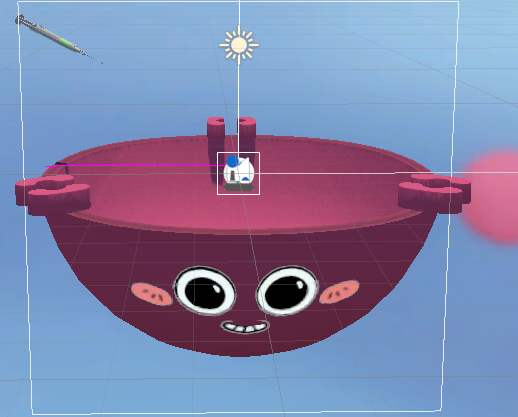
\includegraphics[width=4cm, height=3cm]{asset1.png}
				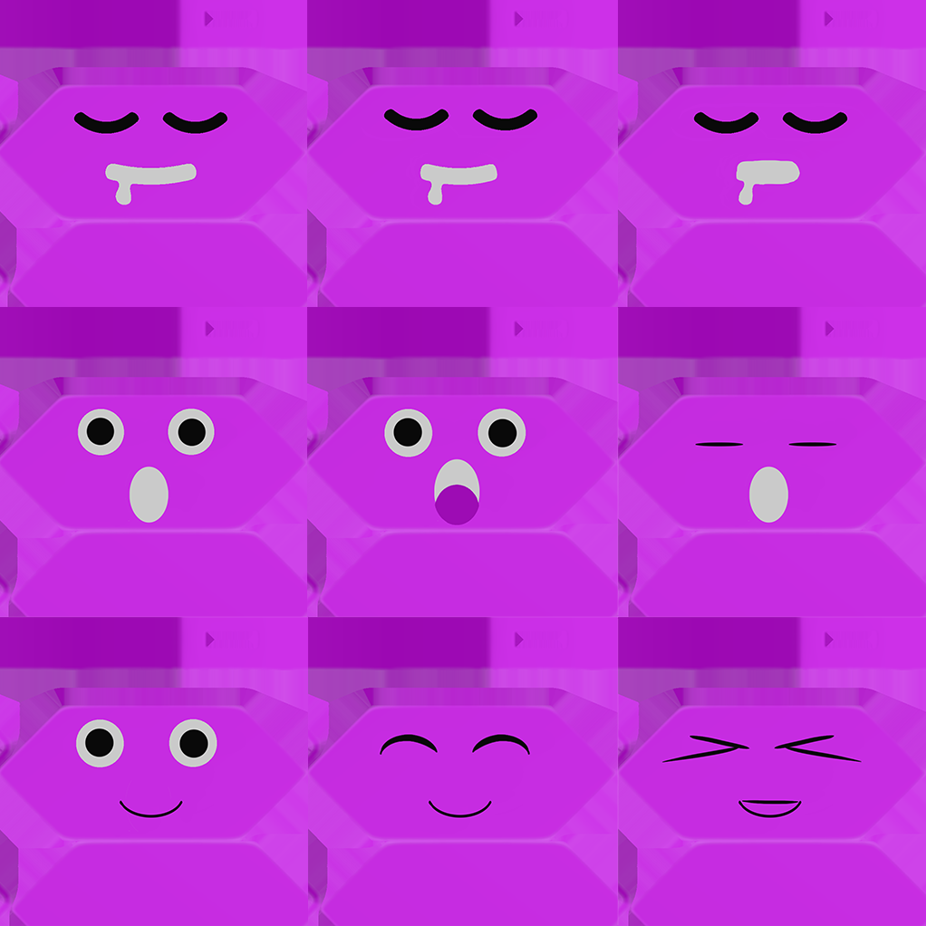
\includegraphics[width=4cm, height=3cm]{asset2.png}
			\end{column}
			\begin{column}{0.33\textwidth}
				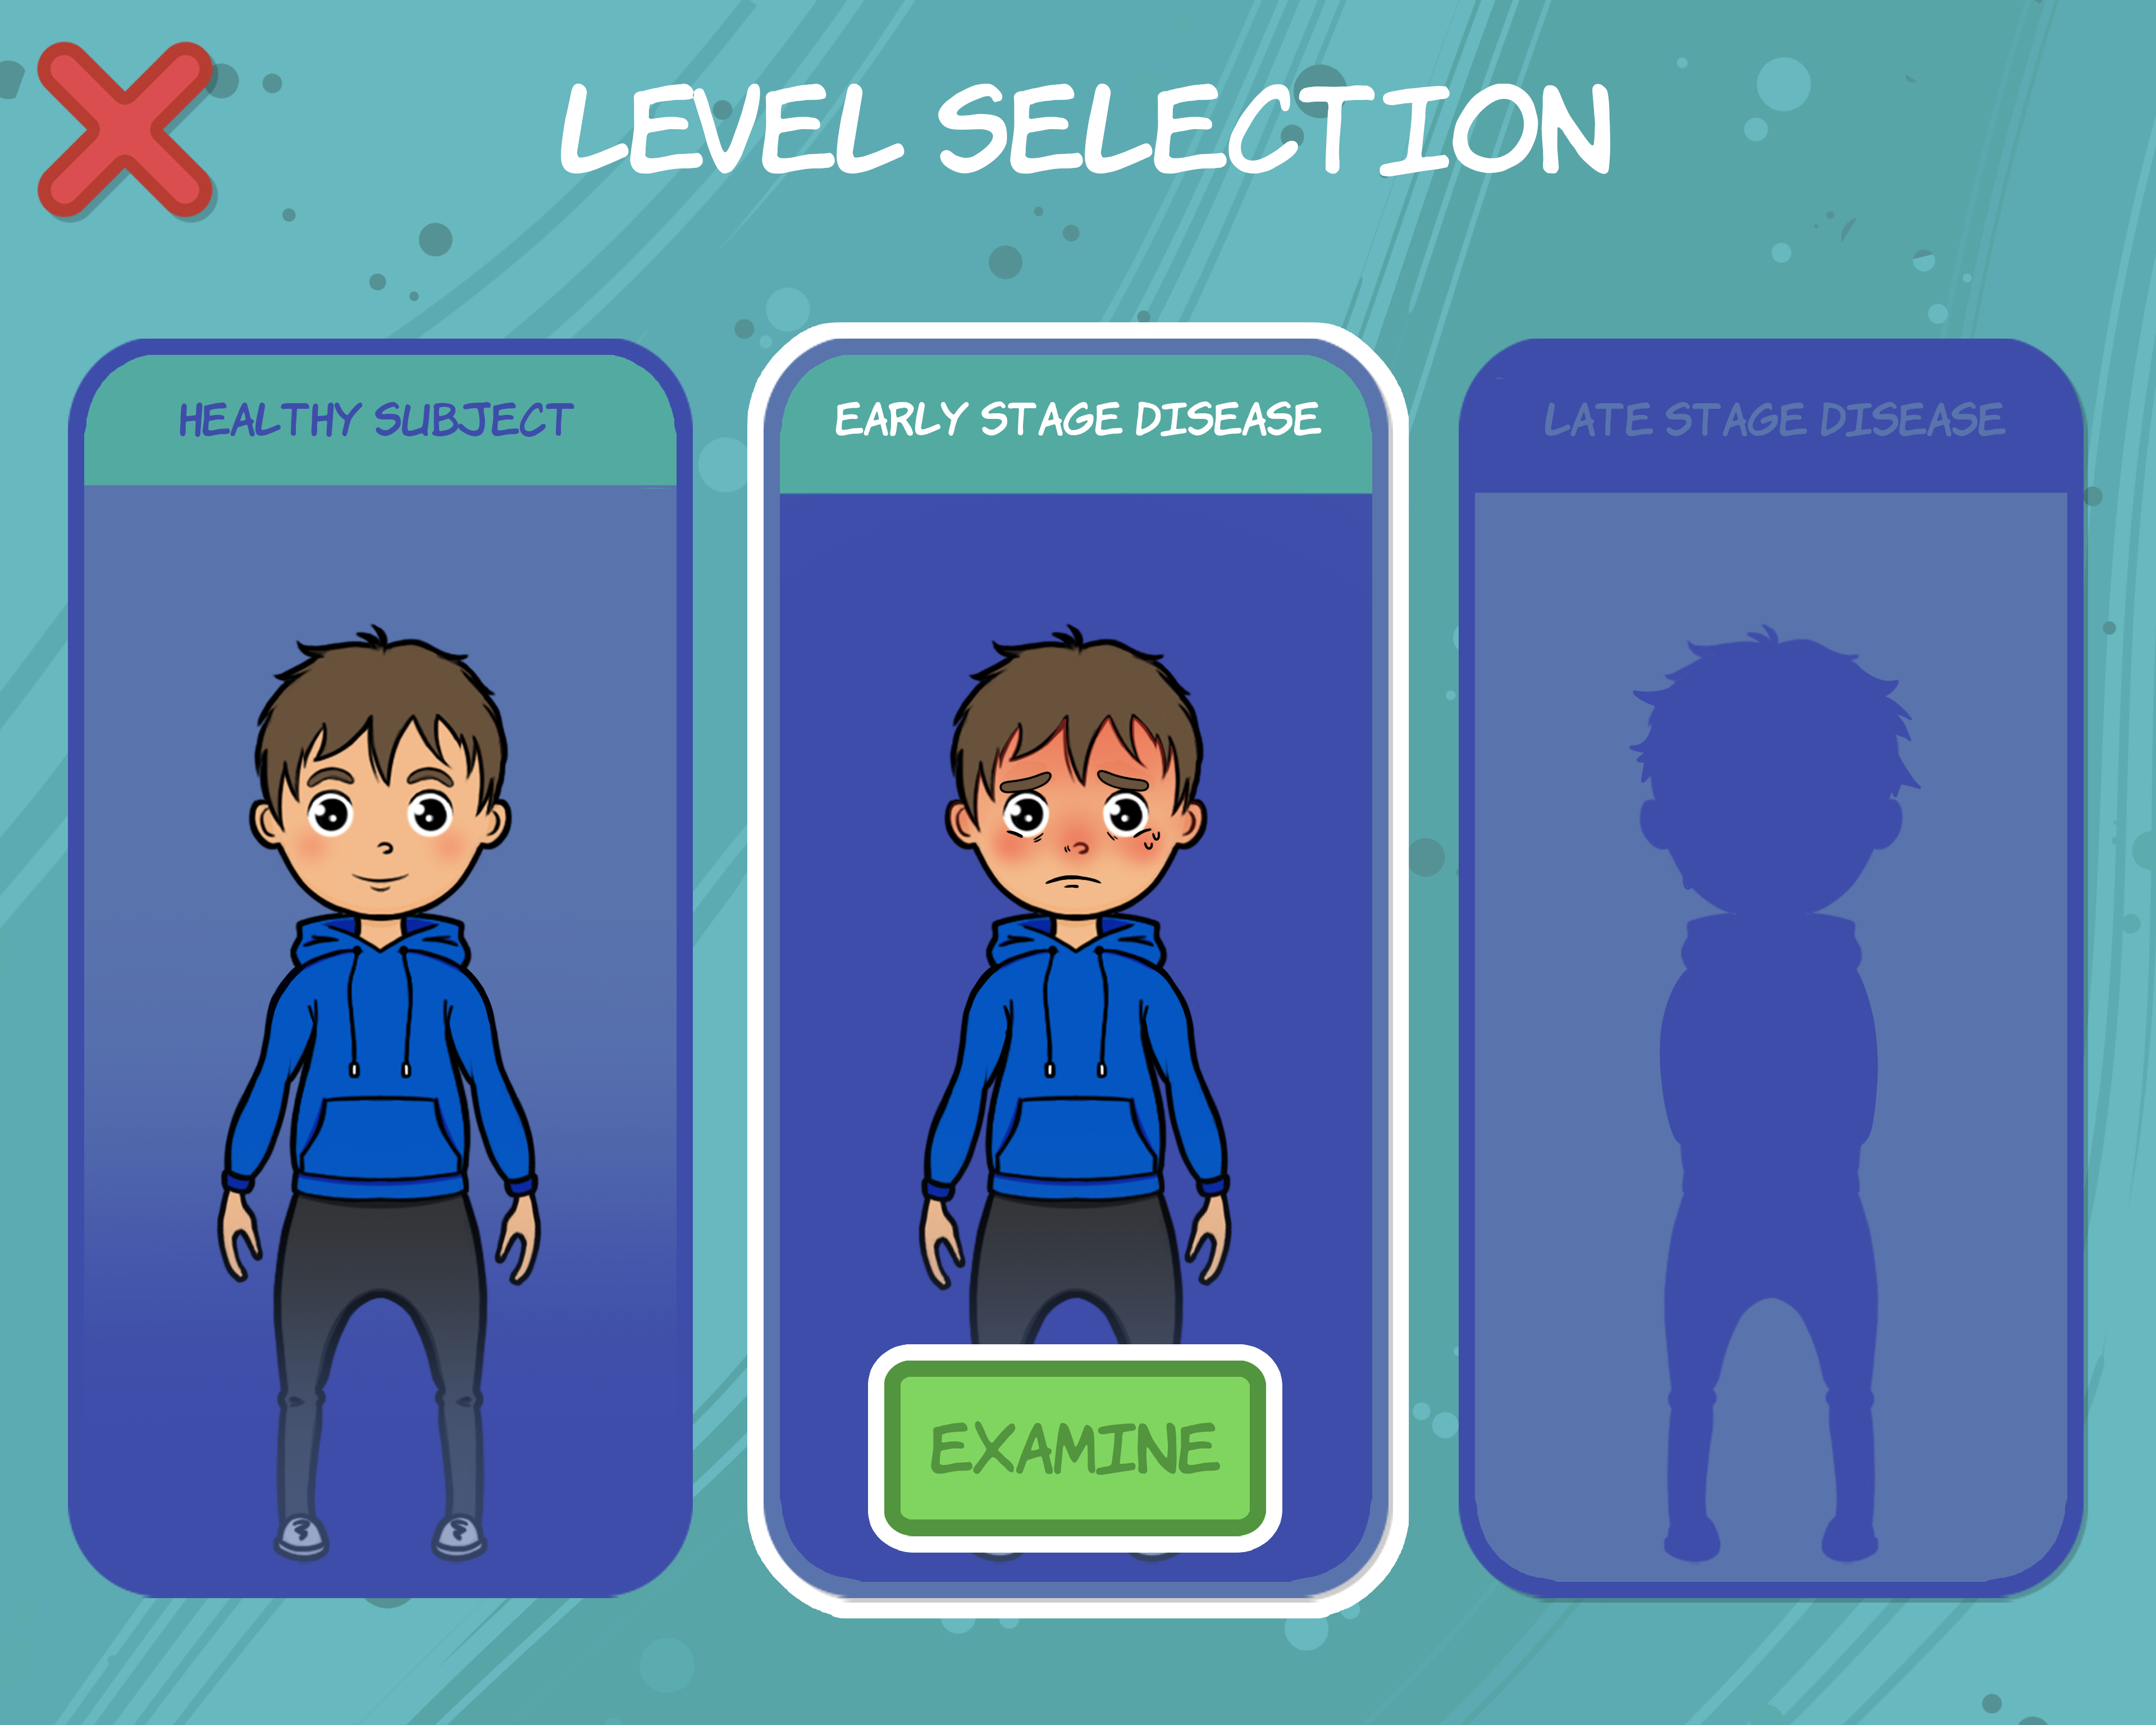
\includegraphics[width=4cm, height=3cm]{asset3.png}
				
\includegraphics[width=4cm, height=3cm]{asset4.png}
			\end{column}
			\begin{column}{0.33\textwidth}
				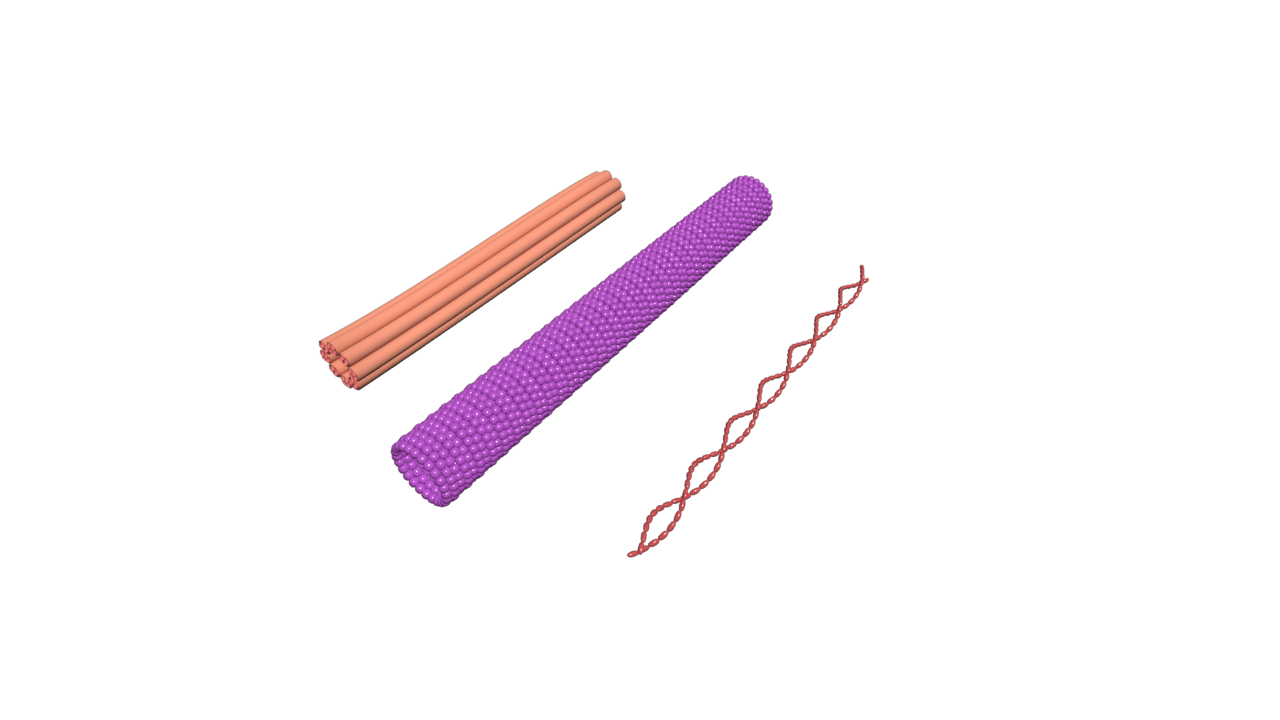
\includegraphics[width=4cm, height=3cm]{asset5.png}
				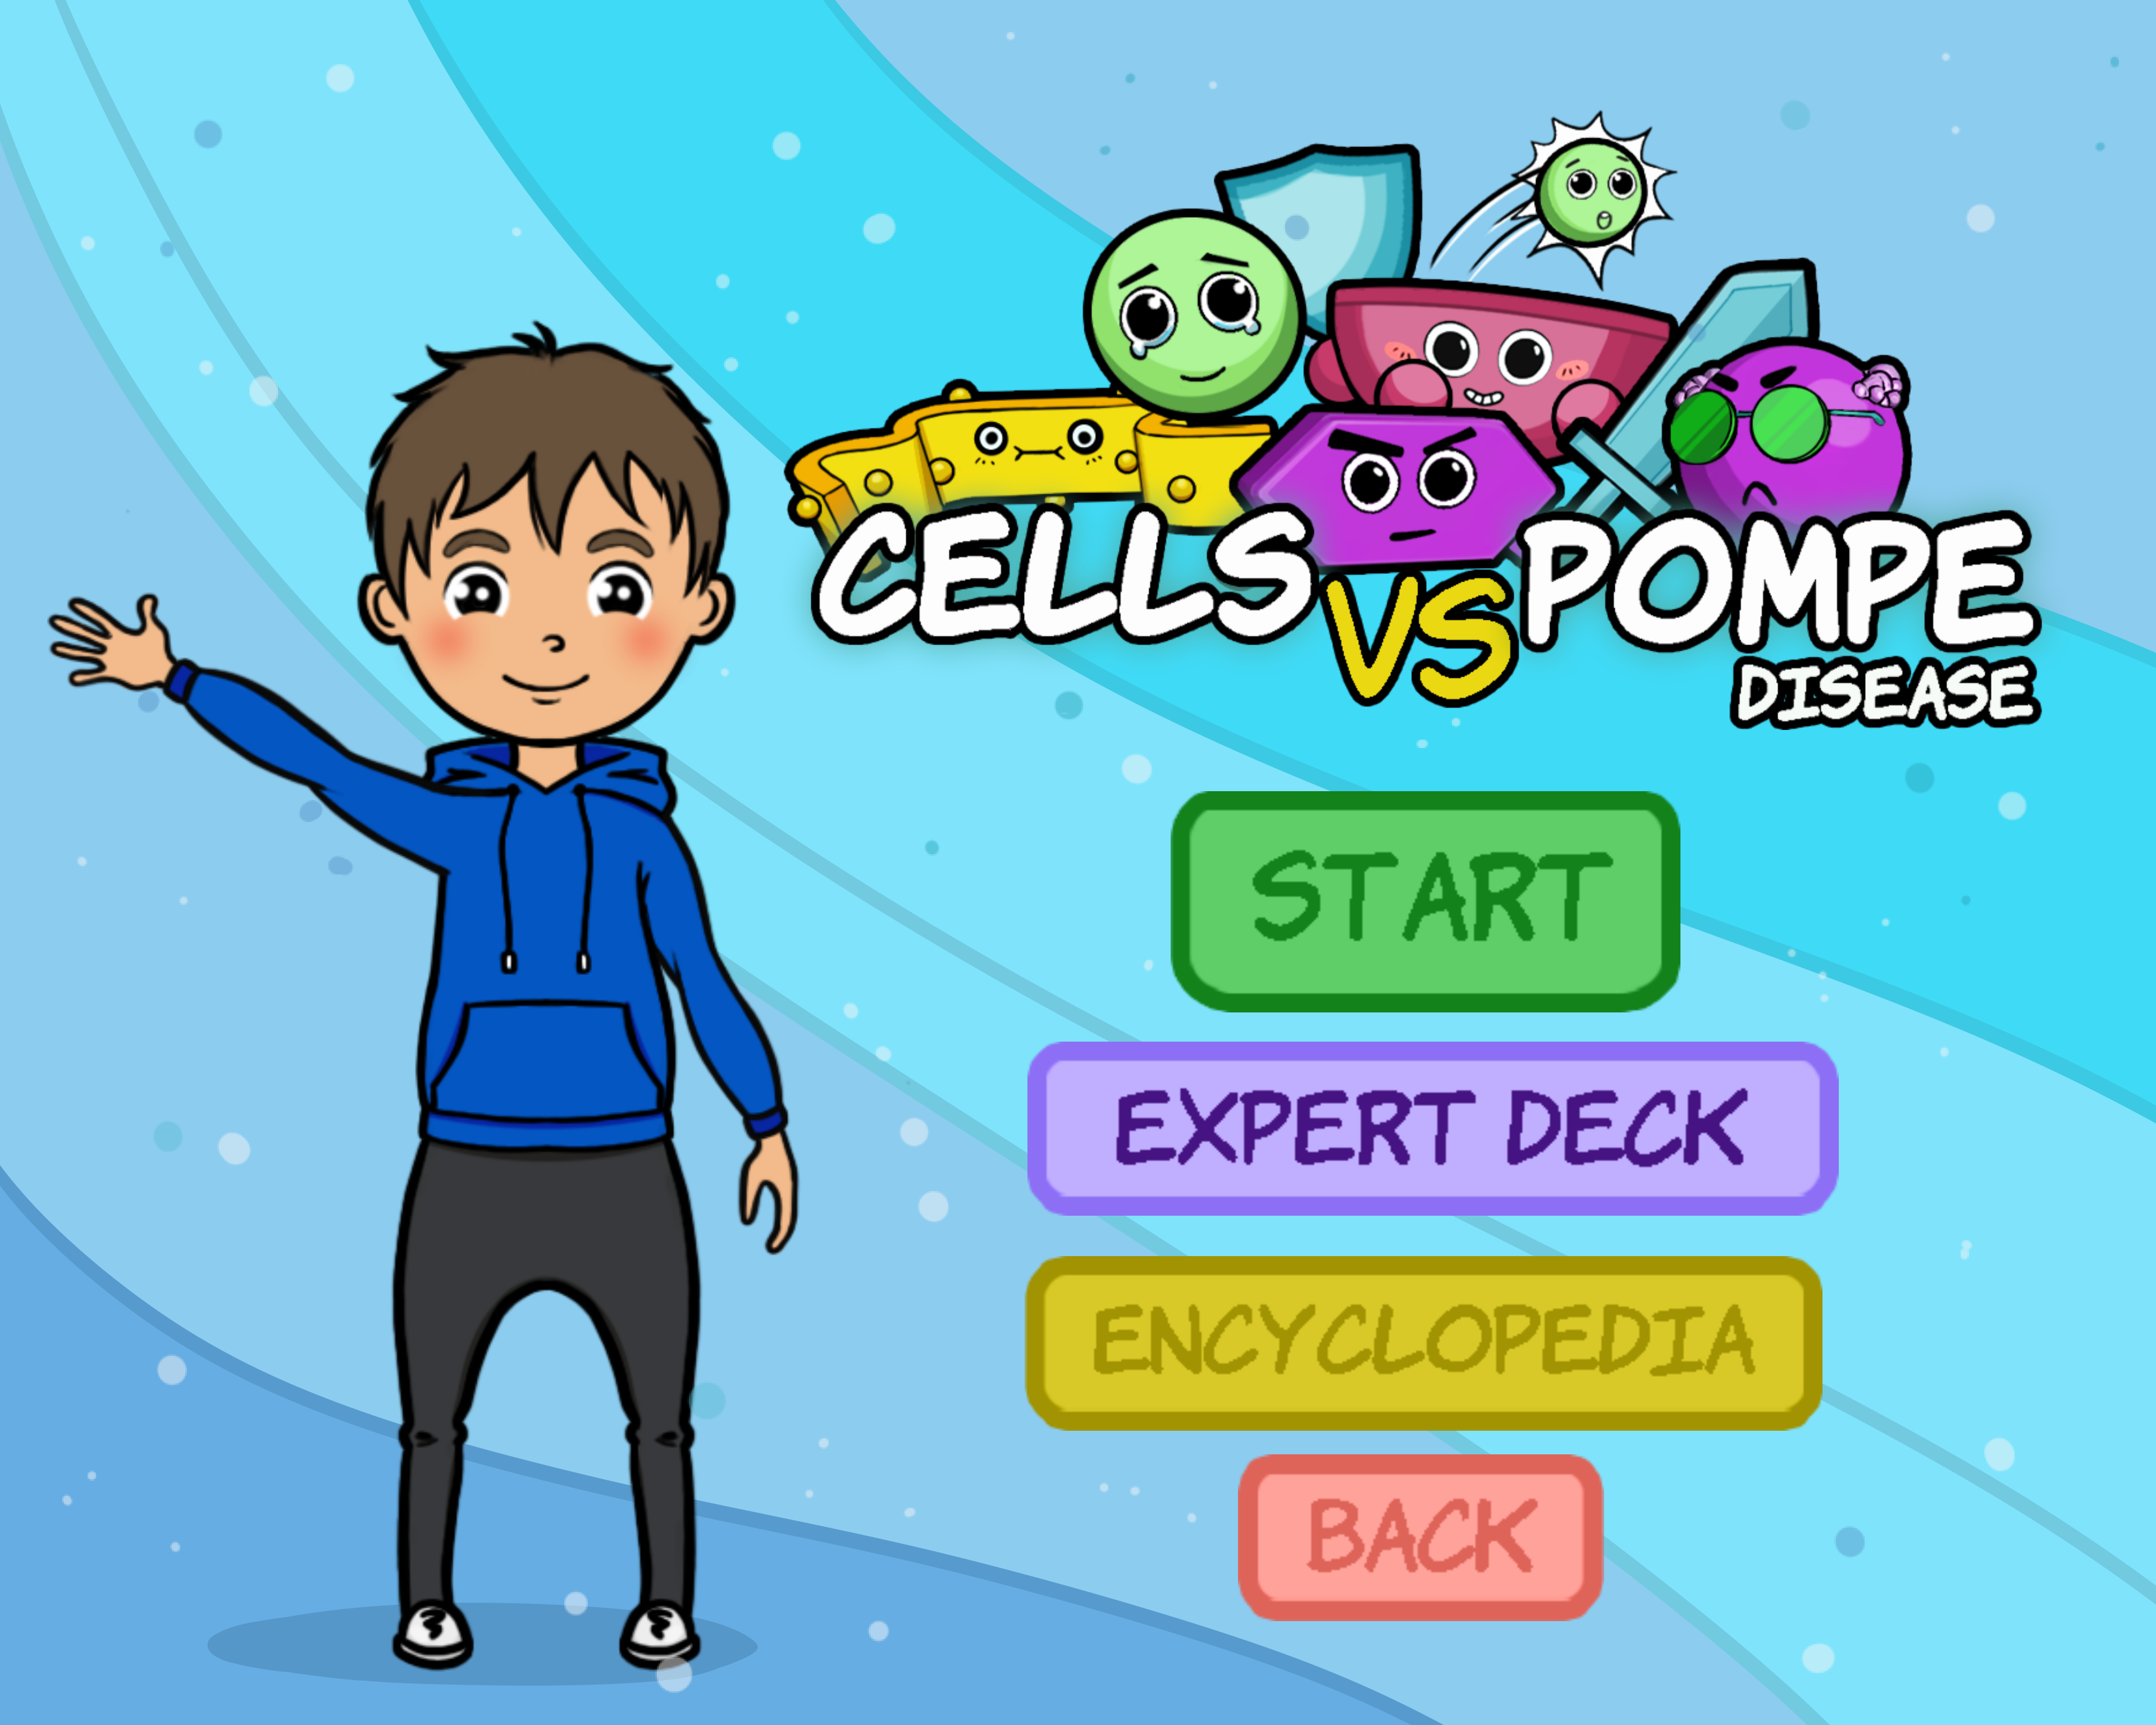
\includegraphics[width=4cm, height=3cm]{asset6.png}
			\end{column}
		\end{columns}		
	\end{frame}

	\begin{frame}{Some Gameplay}
		\centering
		\movie[width=10cm,height=7cm,showcontrols=true]{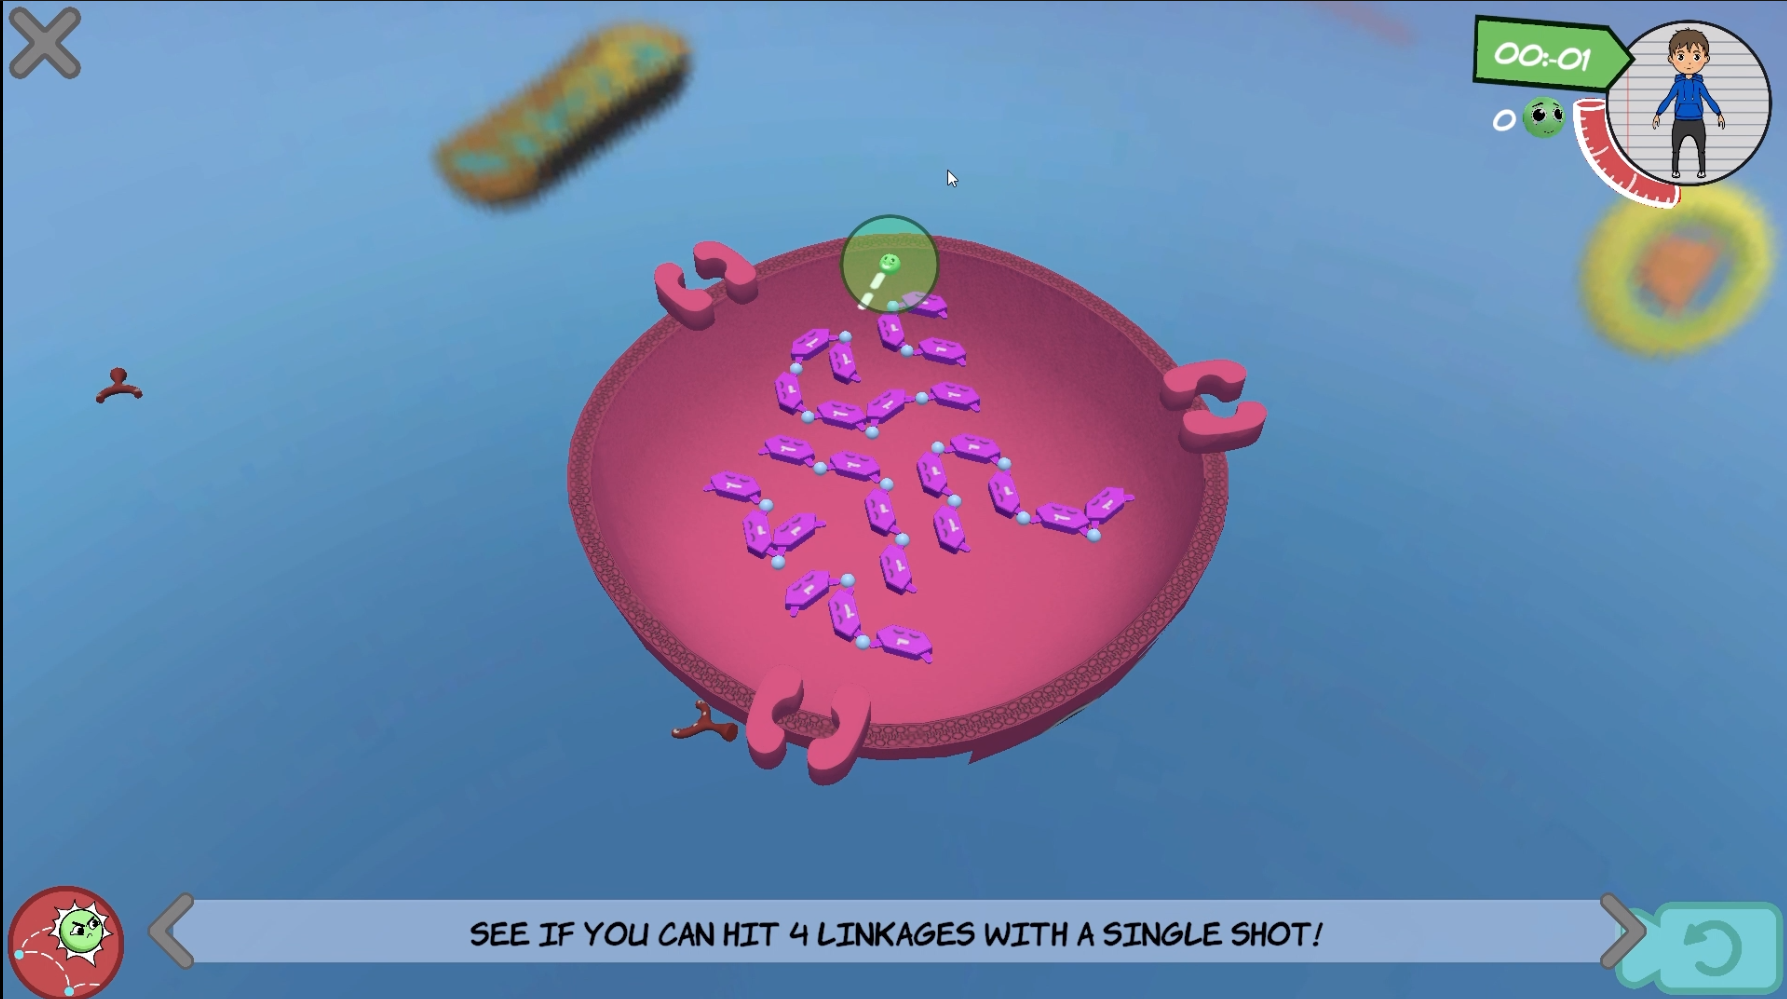
\includegraphics[width=10cm, height=7cm]{pompe_thumbnail.png}}{pompe_trimmed.mp4}
	\end{frame}

	%%% EXPLAIN NSSE SURVEY A BIT
	%%% WHEN YOU TALK MENTION THAT THEY DID THIS SURVEY AFTER PLAYING THE GAME IN CLASS
	\begin{frame}{Collecting Student Feedback}
		\begin{columns}
			\begin{column}{0.45\textwidth}
				
\includegraphics[width=5cm, height=2cm]{nsse.png}
			\end{column}
			\begin{column}{0.5\textwidth}
				\begin{itemize}
					\item NSSE survey questions assess the extent to which students engage in educational practices in the context of higher levels of learning \newline
					\item 150 participants enrolled in BIO1A03 were asked 14 questions regarding opinions and attitudes on their current undergraduate education, as well as feedback on the use of `Cells at War' for learning in the biology classroom
				\end{itemize}
			\end{column}
		\end{columns}			
		
	\end{frame}

	%%%%RESULTS BEGIN HERE
	\section{Results}
	
	\begin{frame}{How Much Time Students Spend Playing Video Games}
		\begin{center}
		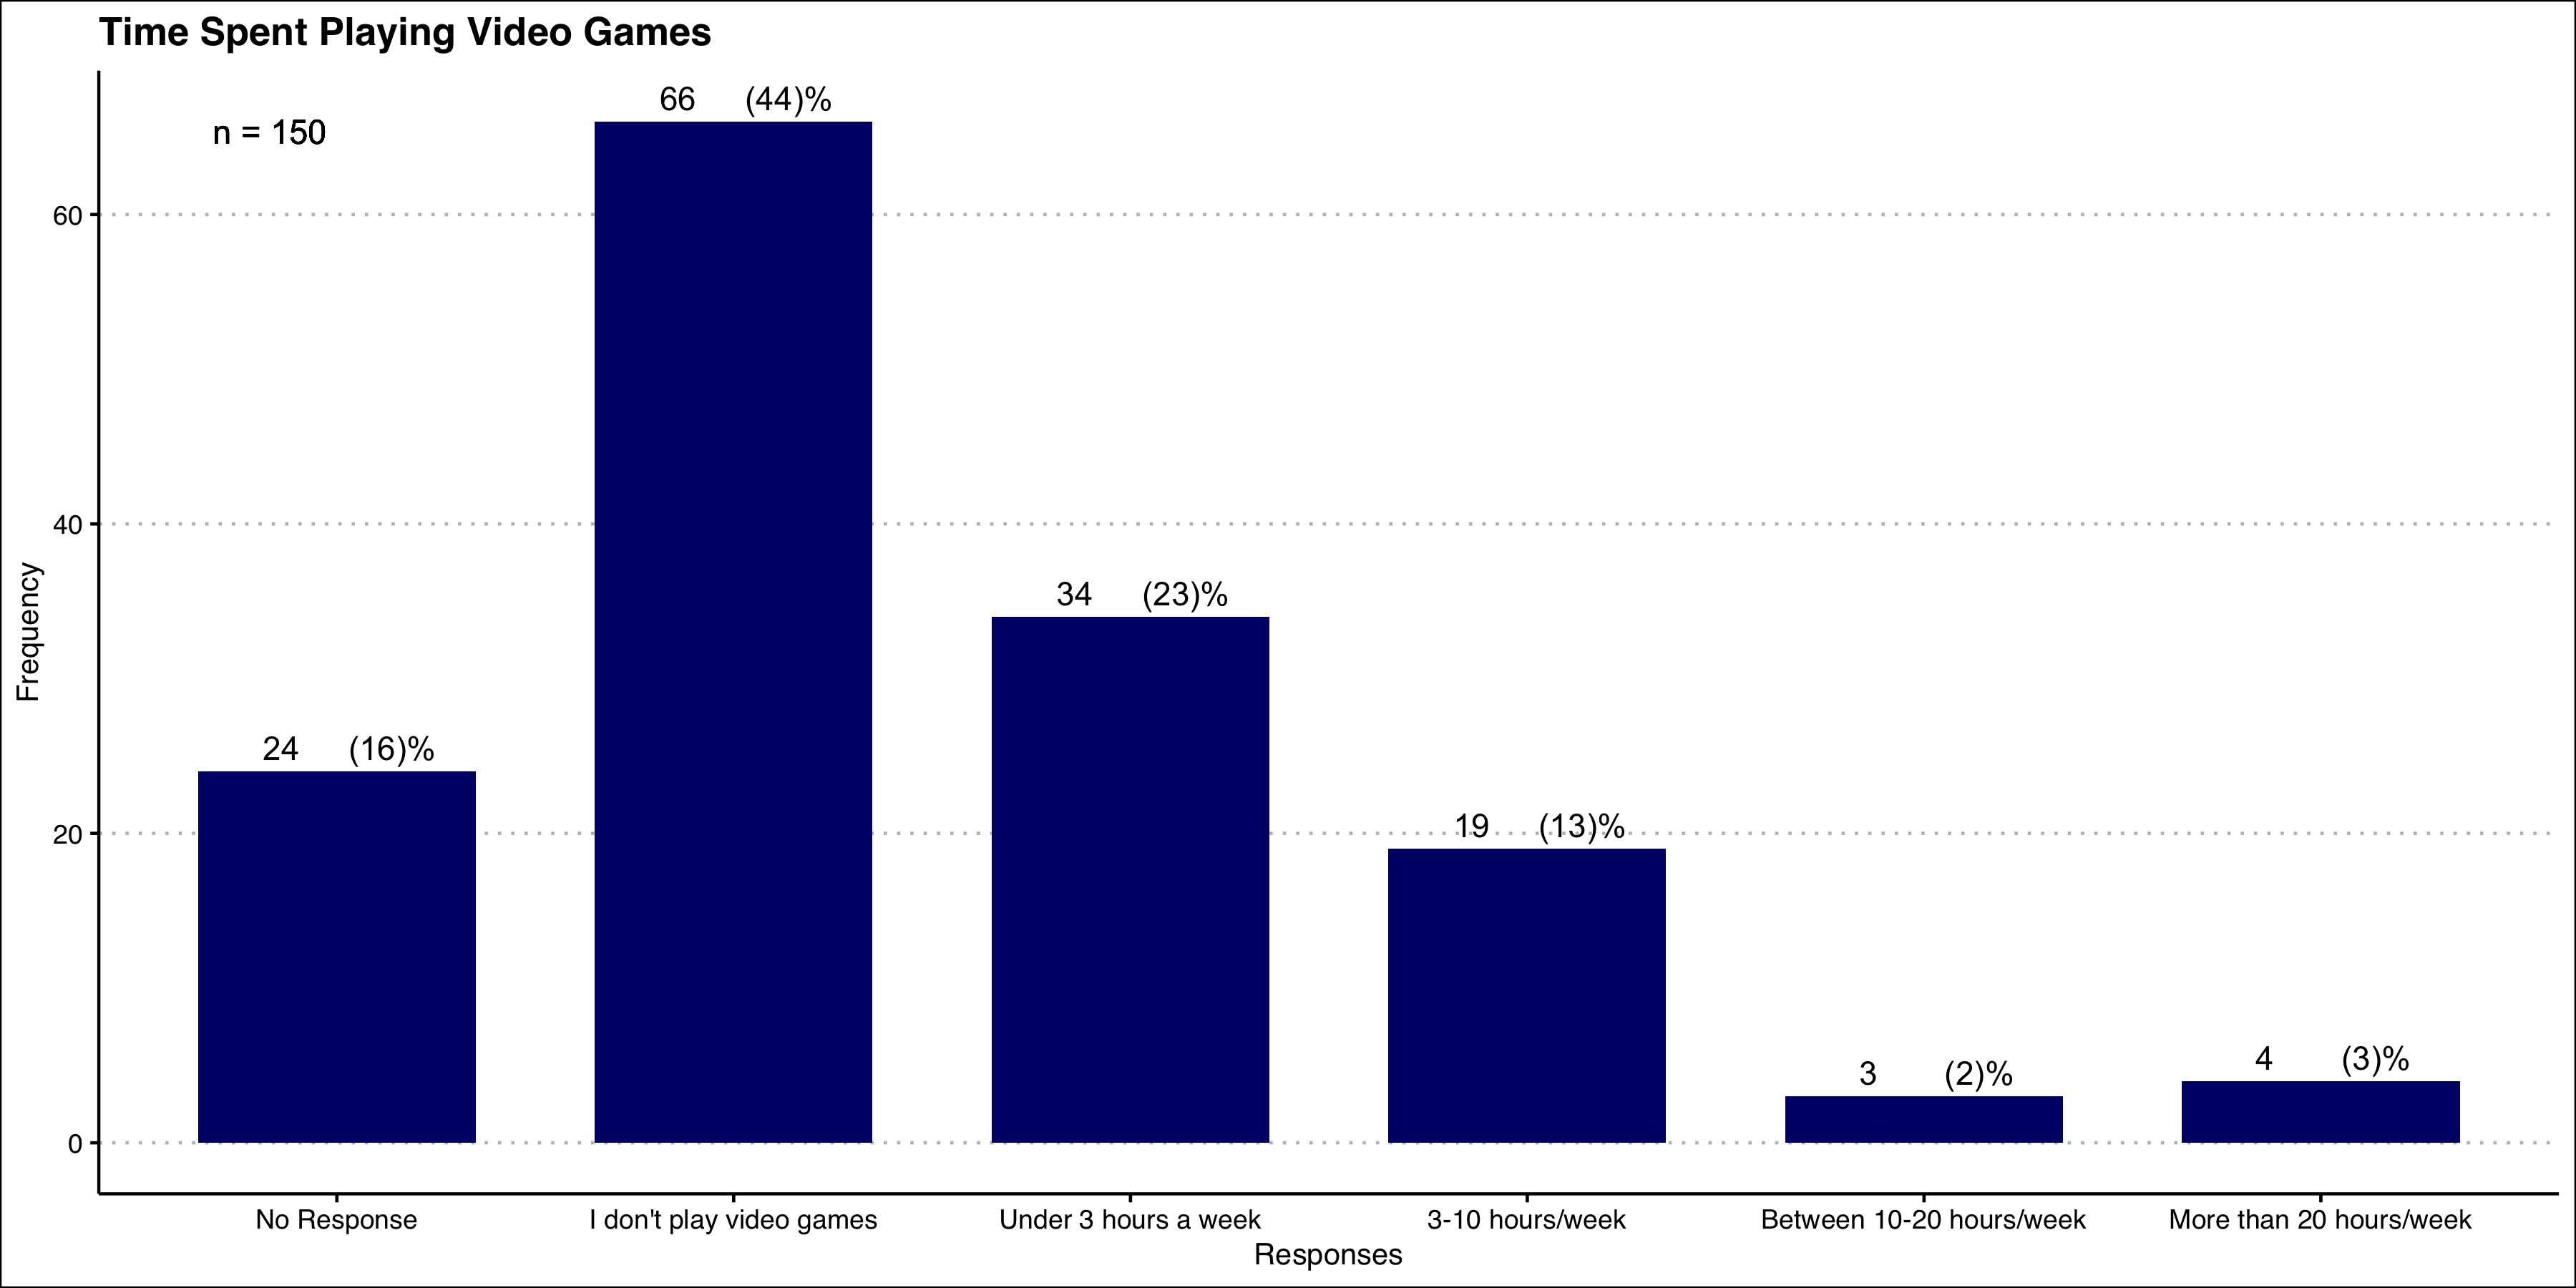
\includegraphics[width=11cm, height=7cm]{time_spent_playing_videogames.jpg}
		\end{center}
	\end{frame}

	\begin{frame}{Types of Courses Taken at McMaster University}
		\begin{center}
		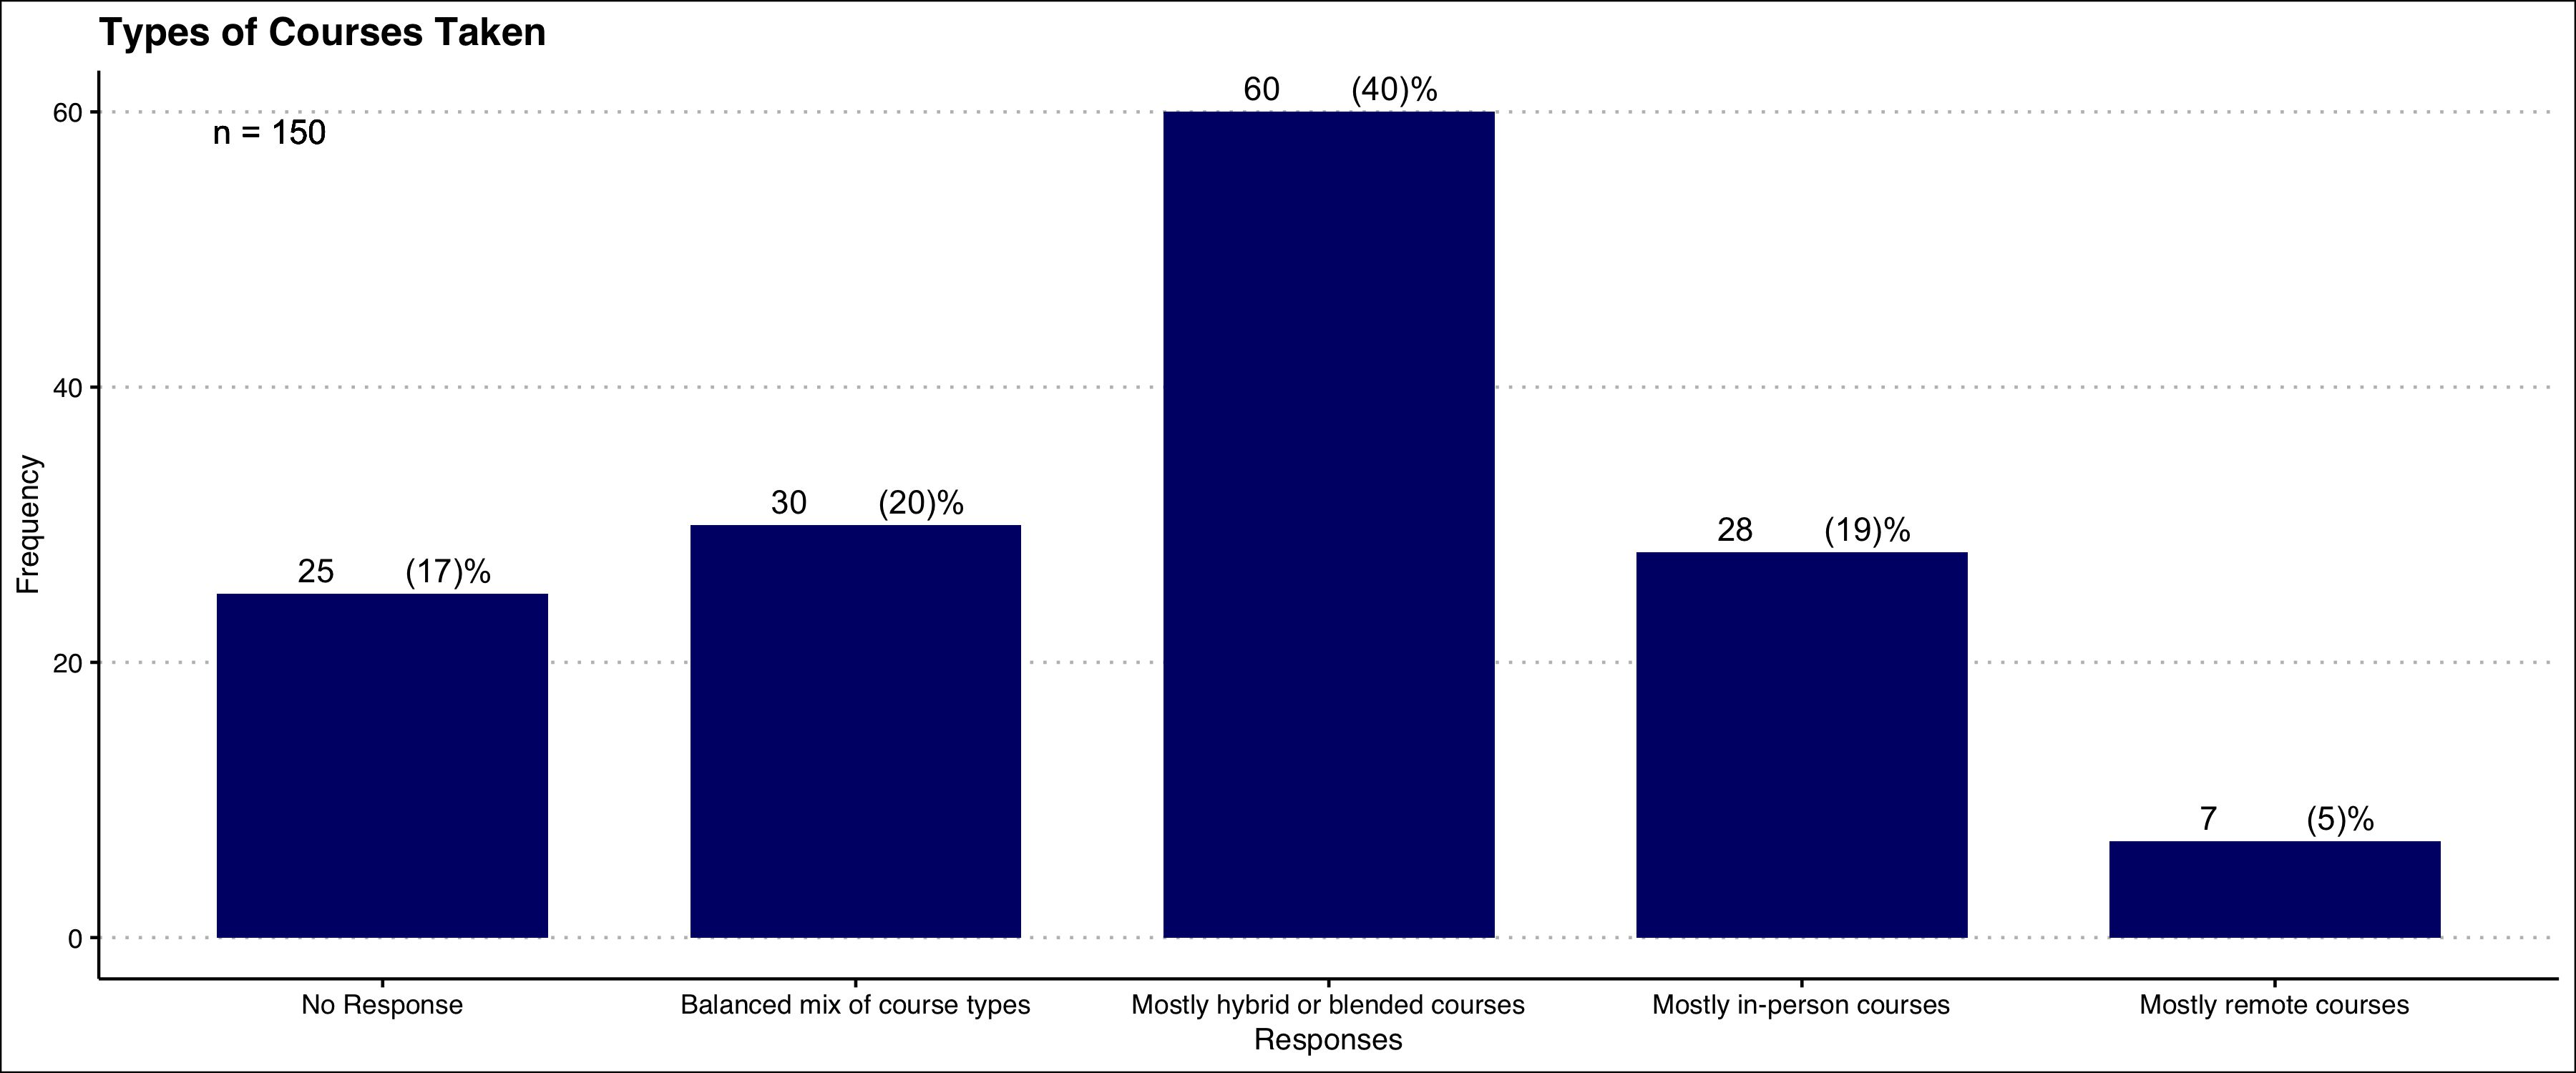
\includegraphics[width=11cm, height=6cm]{types_of_courses_taken.jpg}
		\end{center}
	\end{frame}

	\begin{frame}{During the Current School Year, How Often Have You Done the Following}
		\begin{center}
			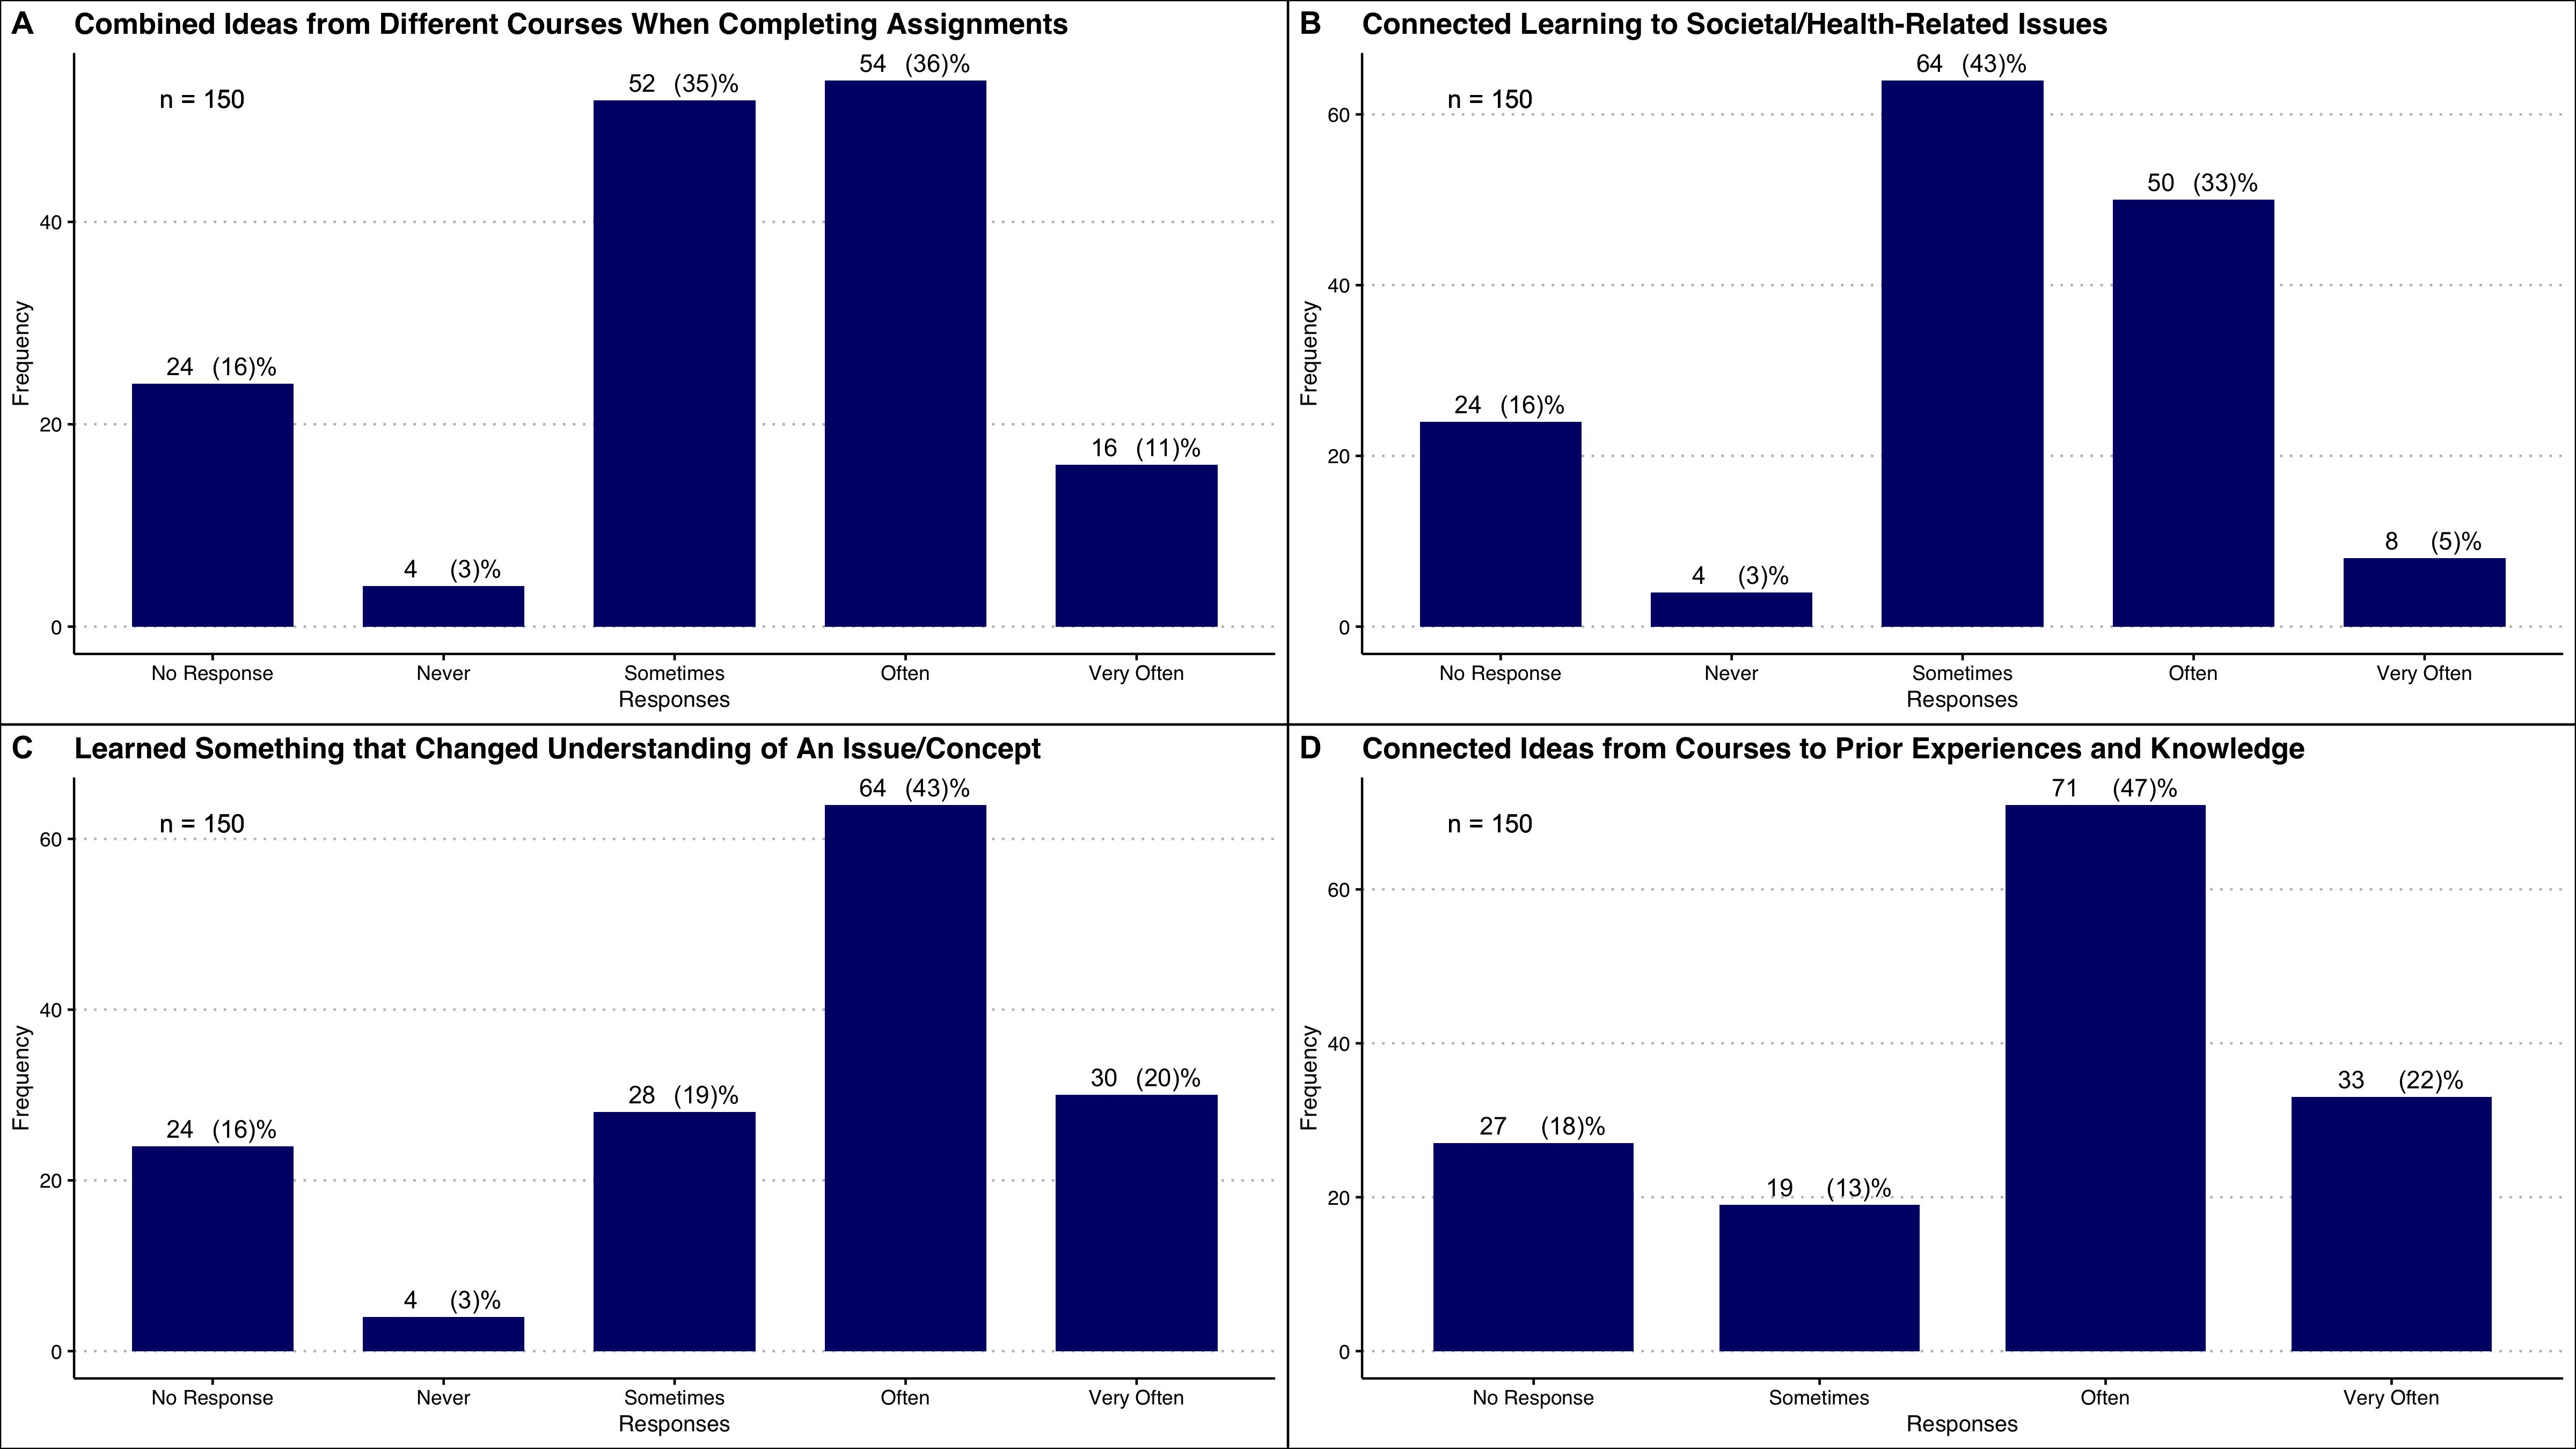
\includegraphics[width=11cm, height=6cm]{how_often_haveyou_done_thefollowing.jpg}
		\end{center}
	\end{frame}

	\begin{frame}{How Could Game-based Learning Help With the Following}
		\begin{center}
			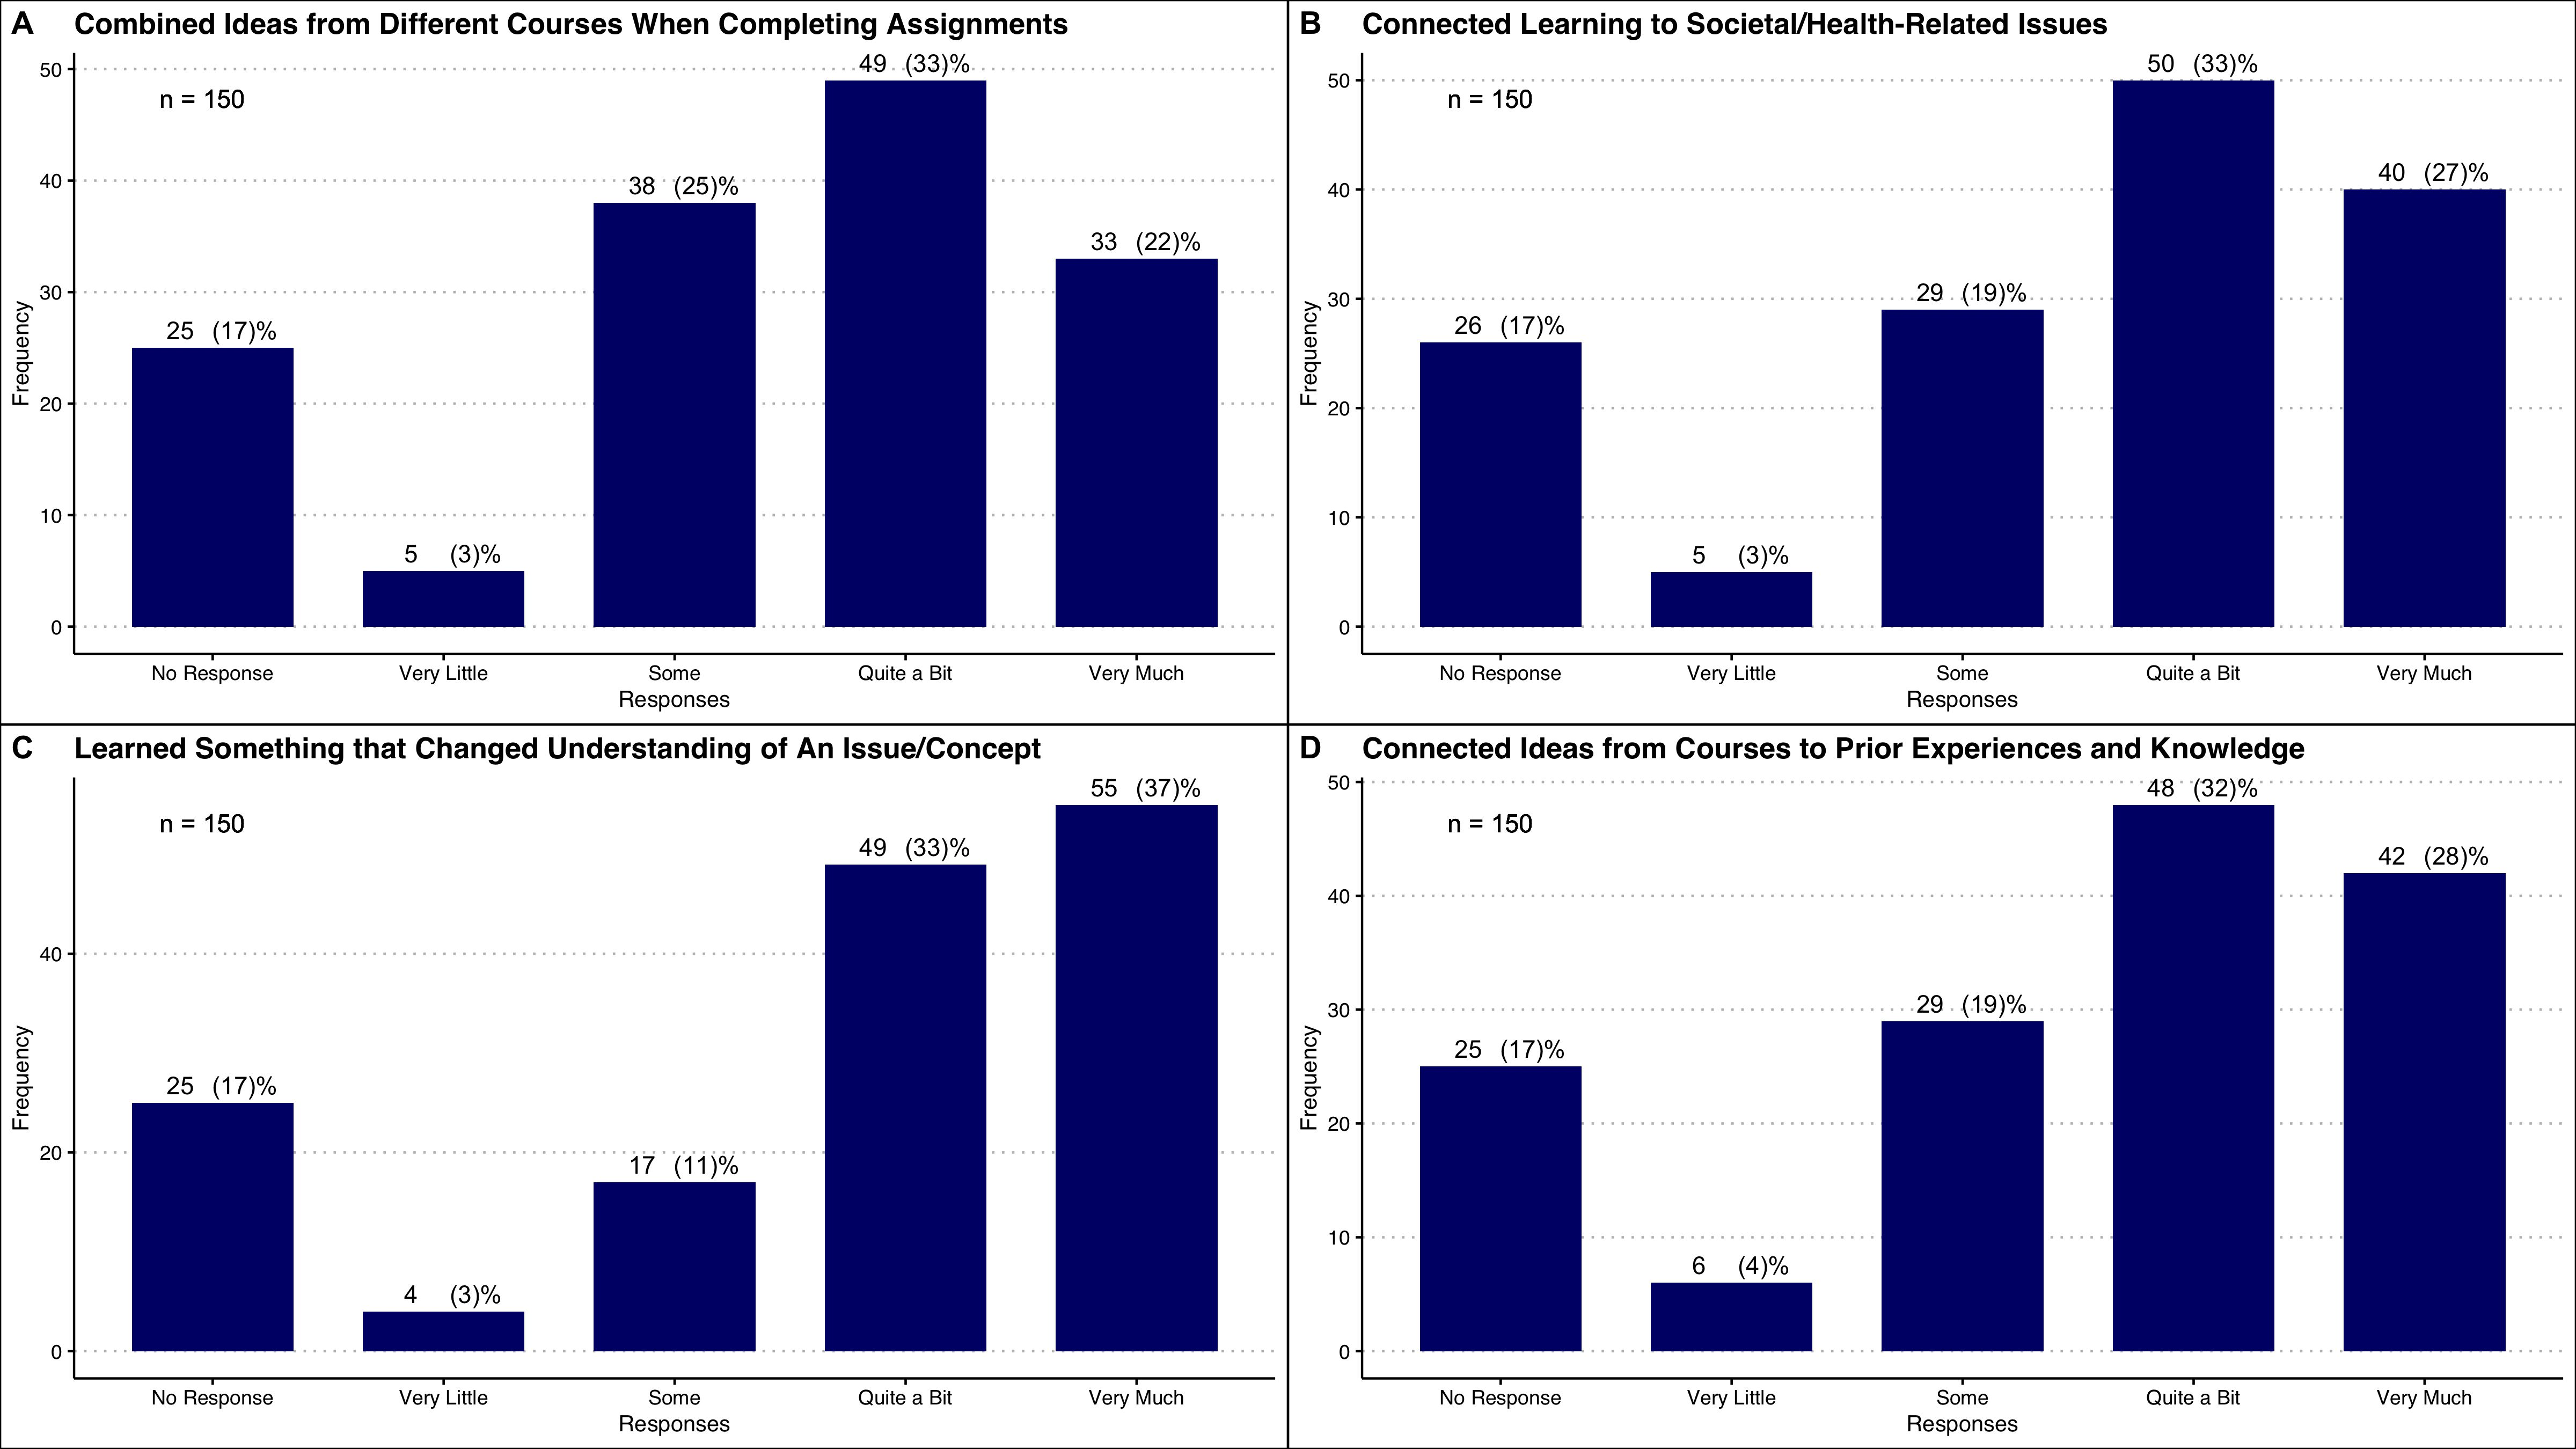
\includegraphics[width=11cm, height=6cm]{how_does_gbl_help_in_science.jpg}
		\end{center}
	\end{frame}

	\begin{frame}{How Much Does Coursework Emphasize the Following}
		\begin{center}
			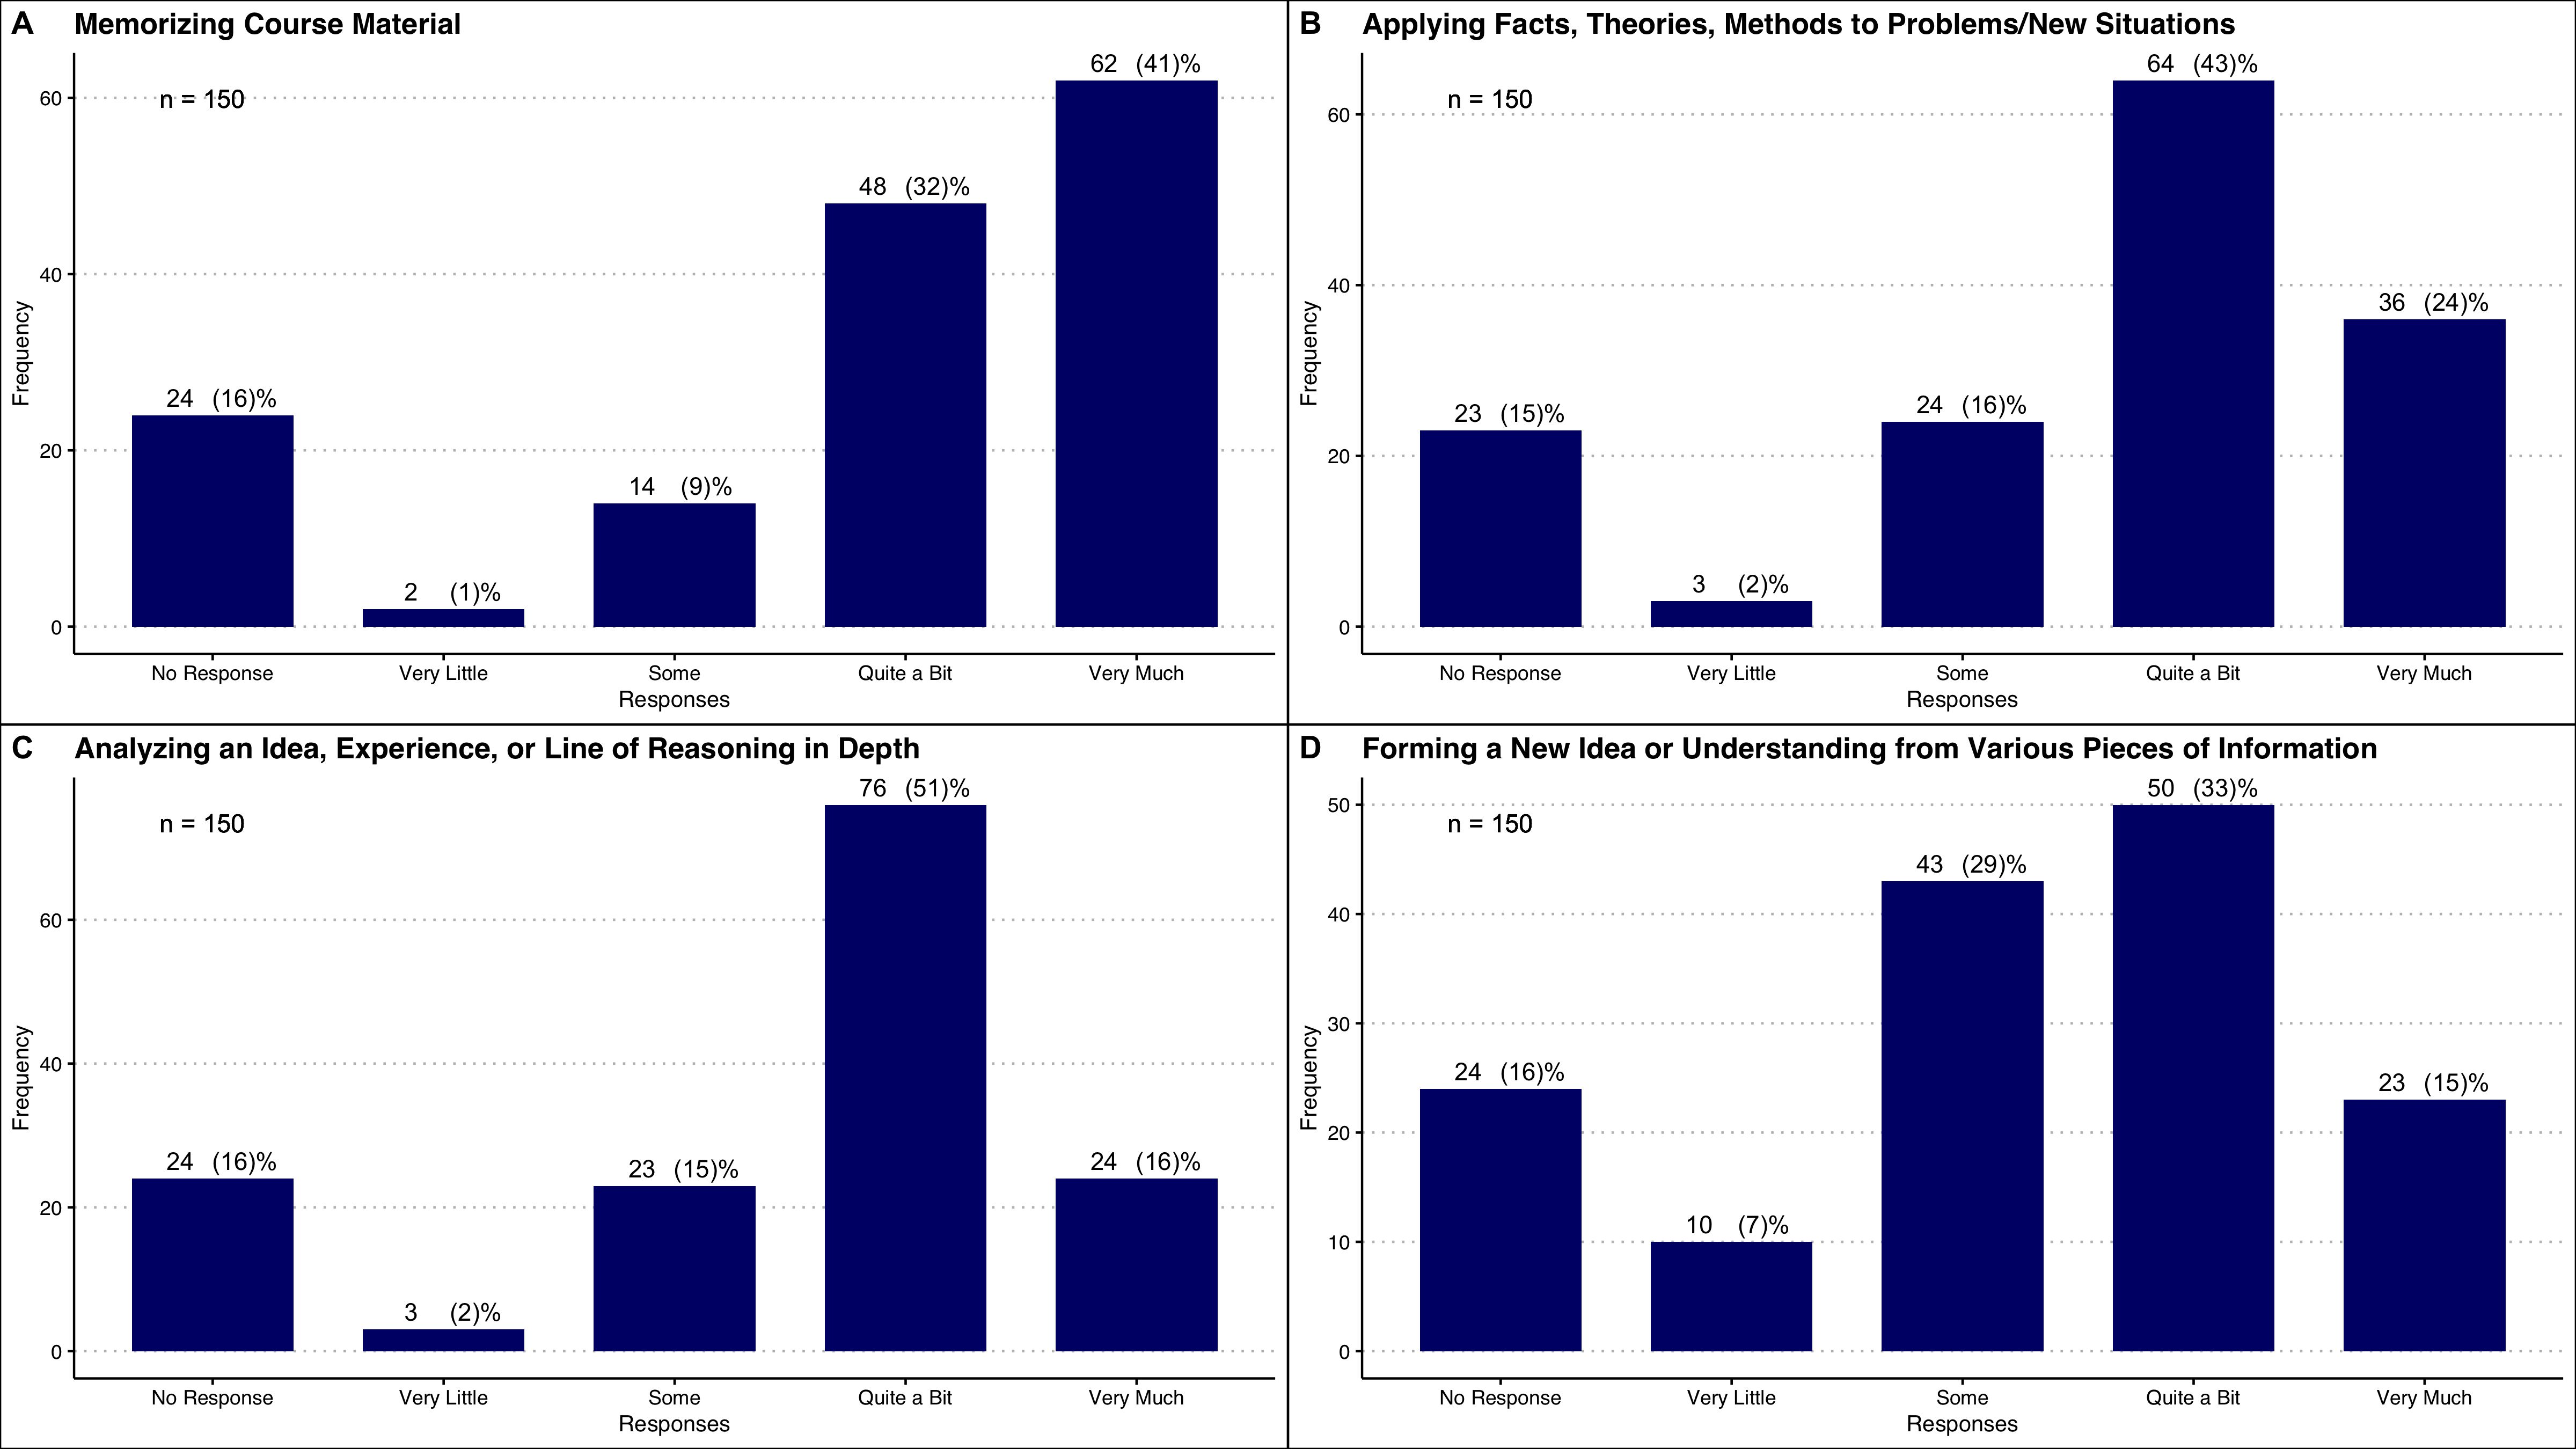
\includegraphics[width=11cm, height=6cm]{howmuch_coursework_emphasized_thefollowing.jpg}
		\end{center}
	\end{frame}

	\begin{frame}{If BIO1A03 Added a GBL Component, How Would it Improve Motivation to do the Following}
		\begin{center}
			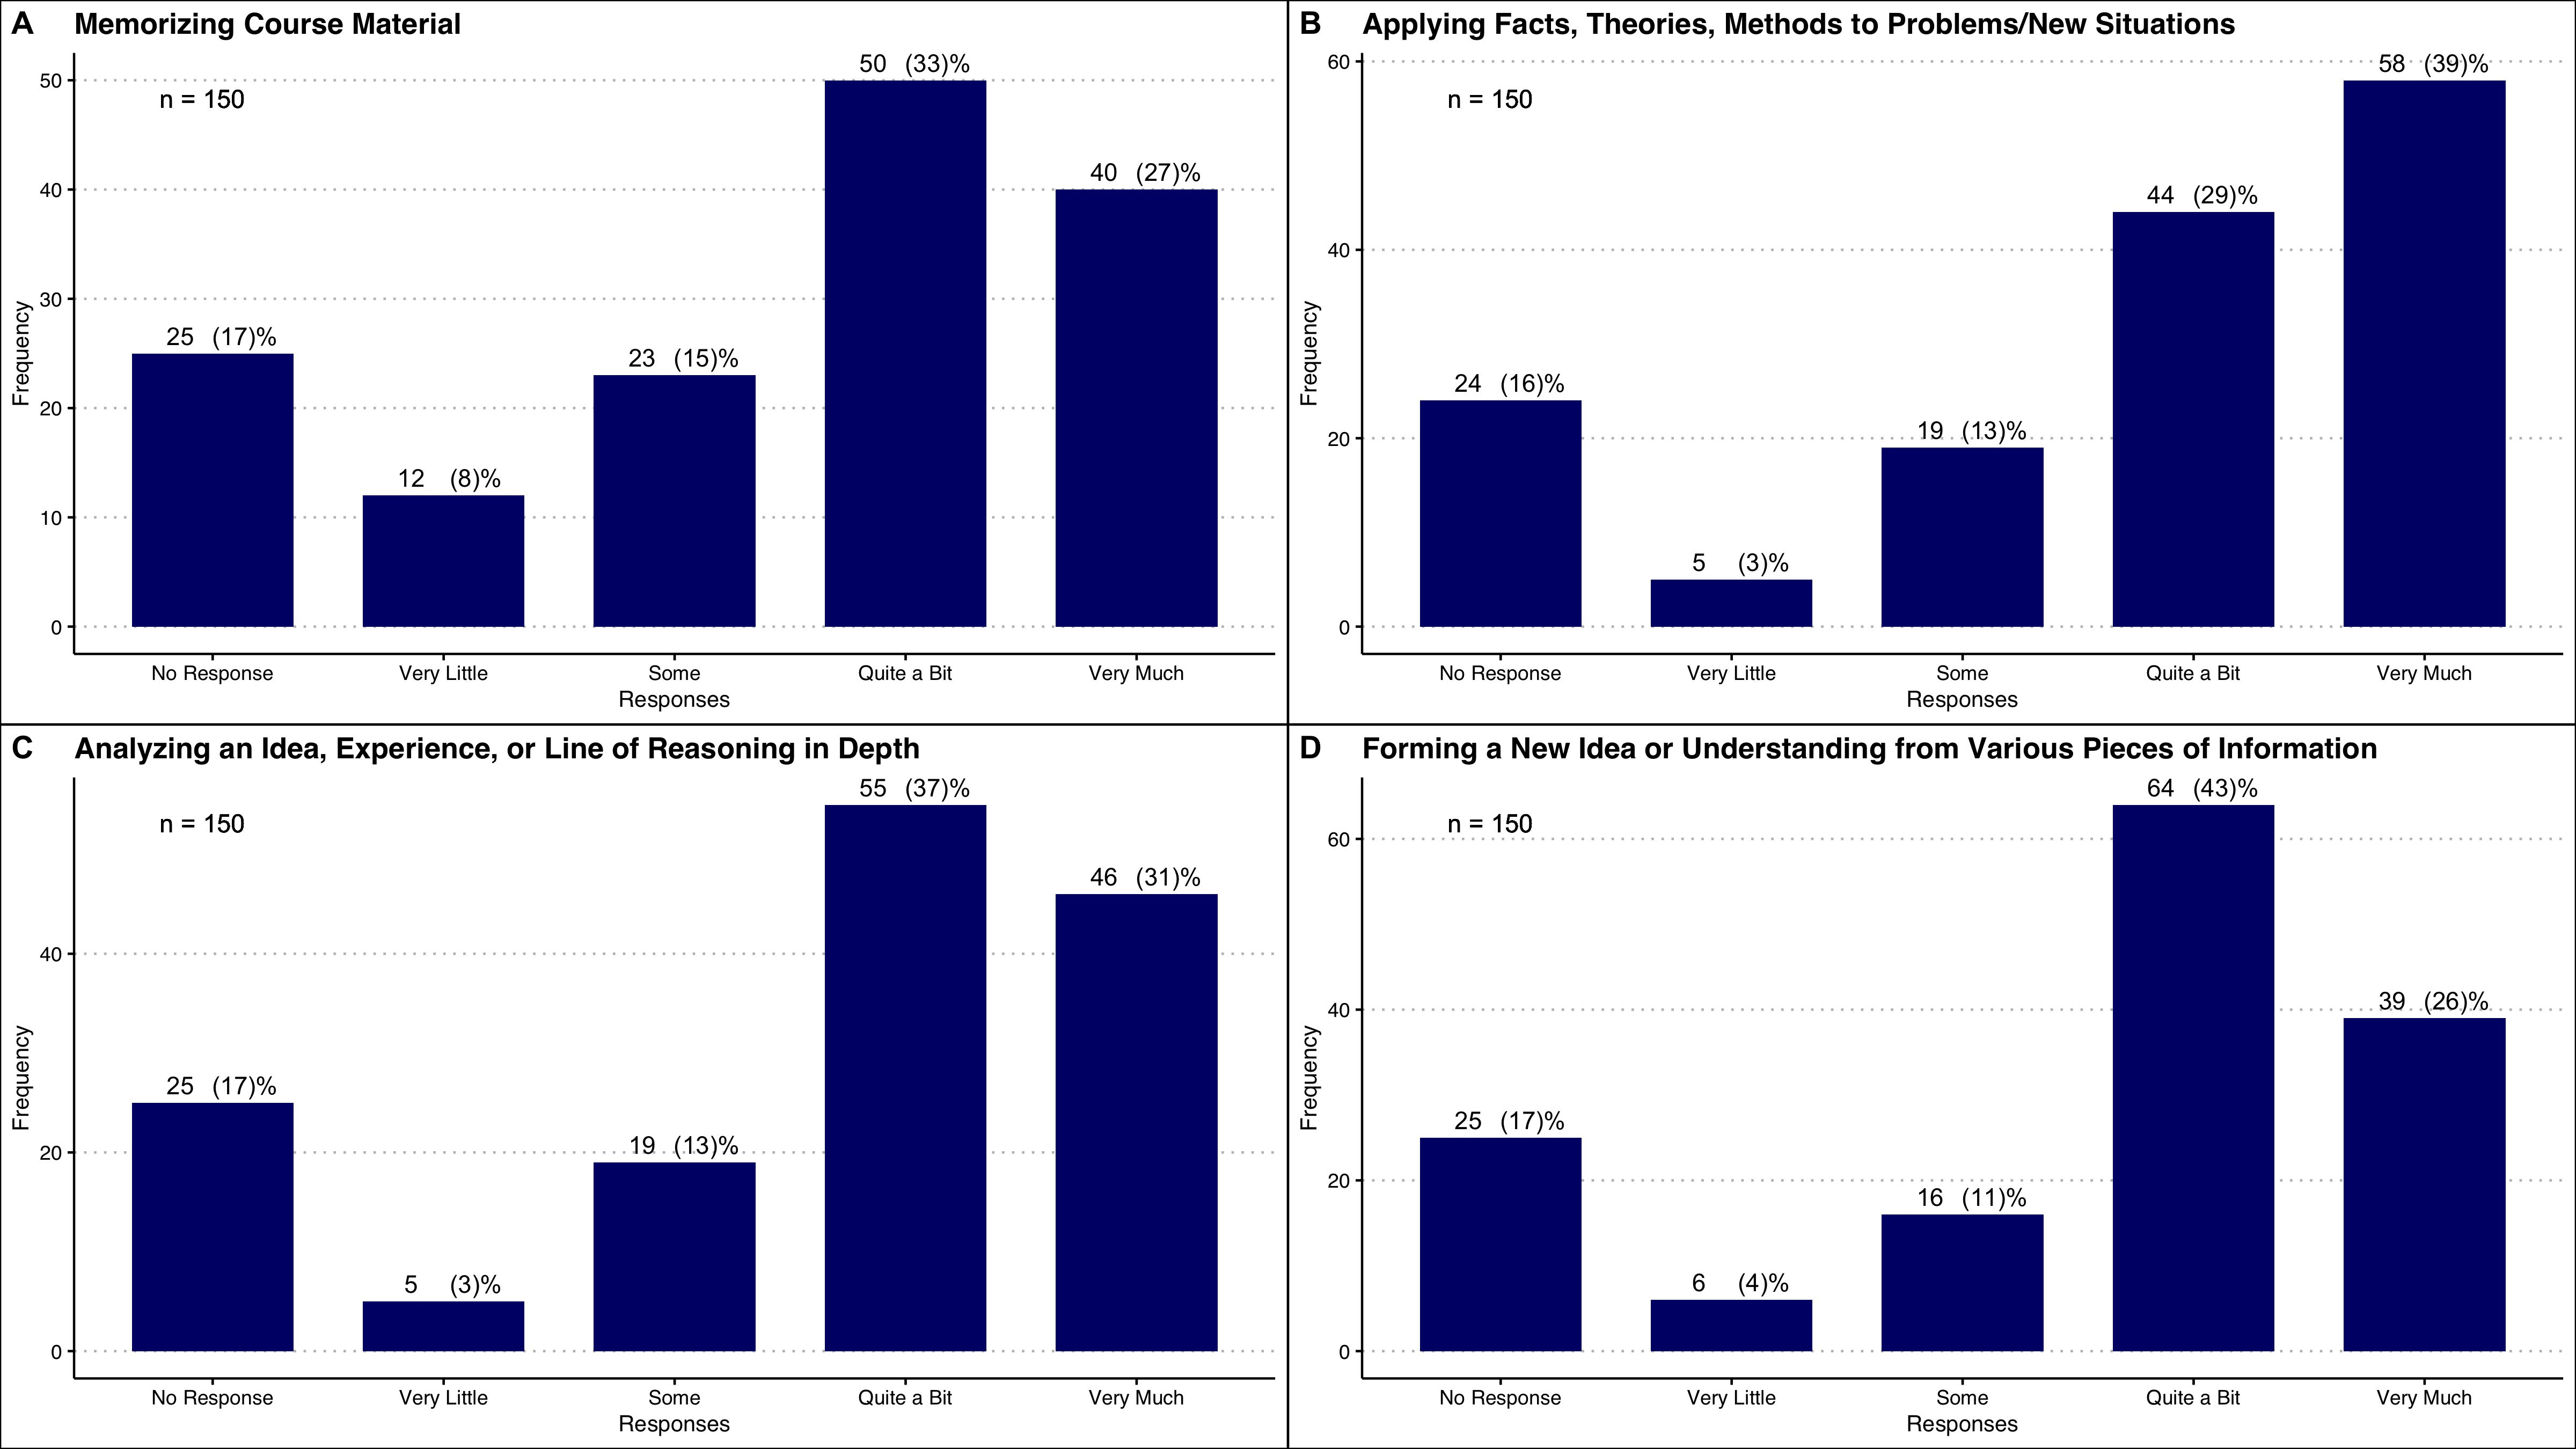
\includegraphics[width=11cm, height=6cm]{ifbio1a03_added_gblcomponent.jpg}
		\end{center}
	\end{frame}

	\begin{frame}{How Likely is it You Would Play Cells at War on Your Own Time To Consolidate Material Taught During Class}
		\begin{center}
			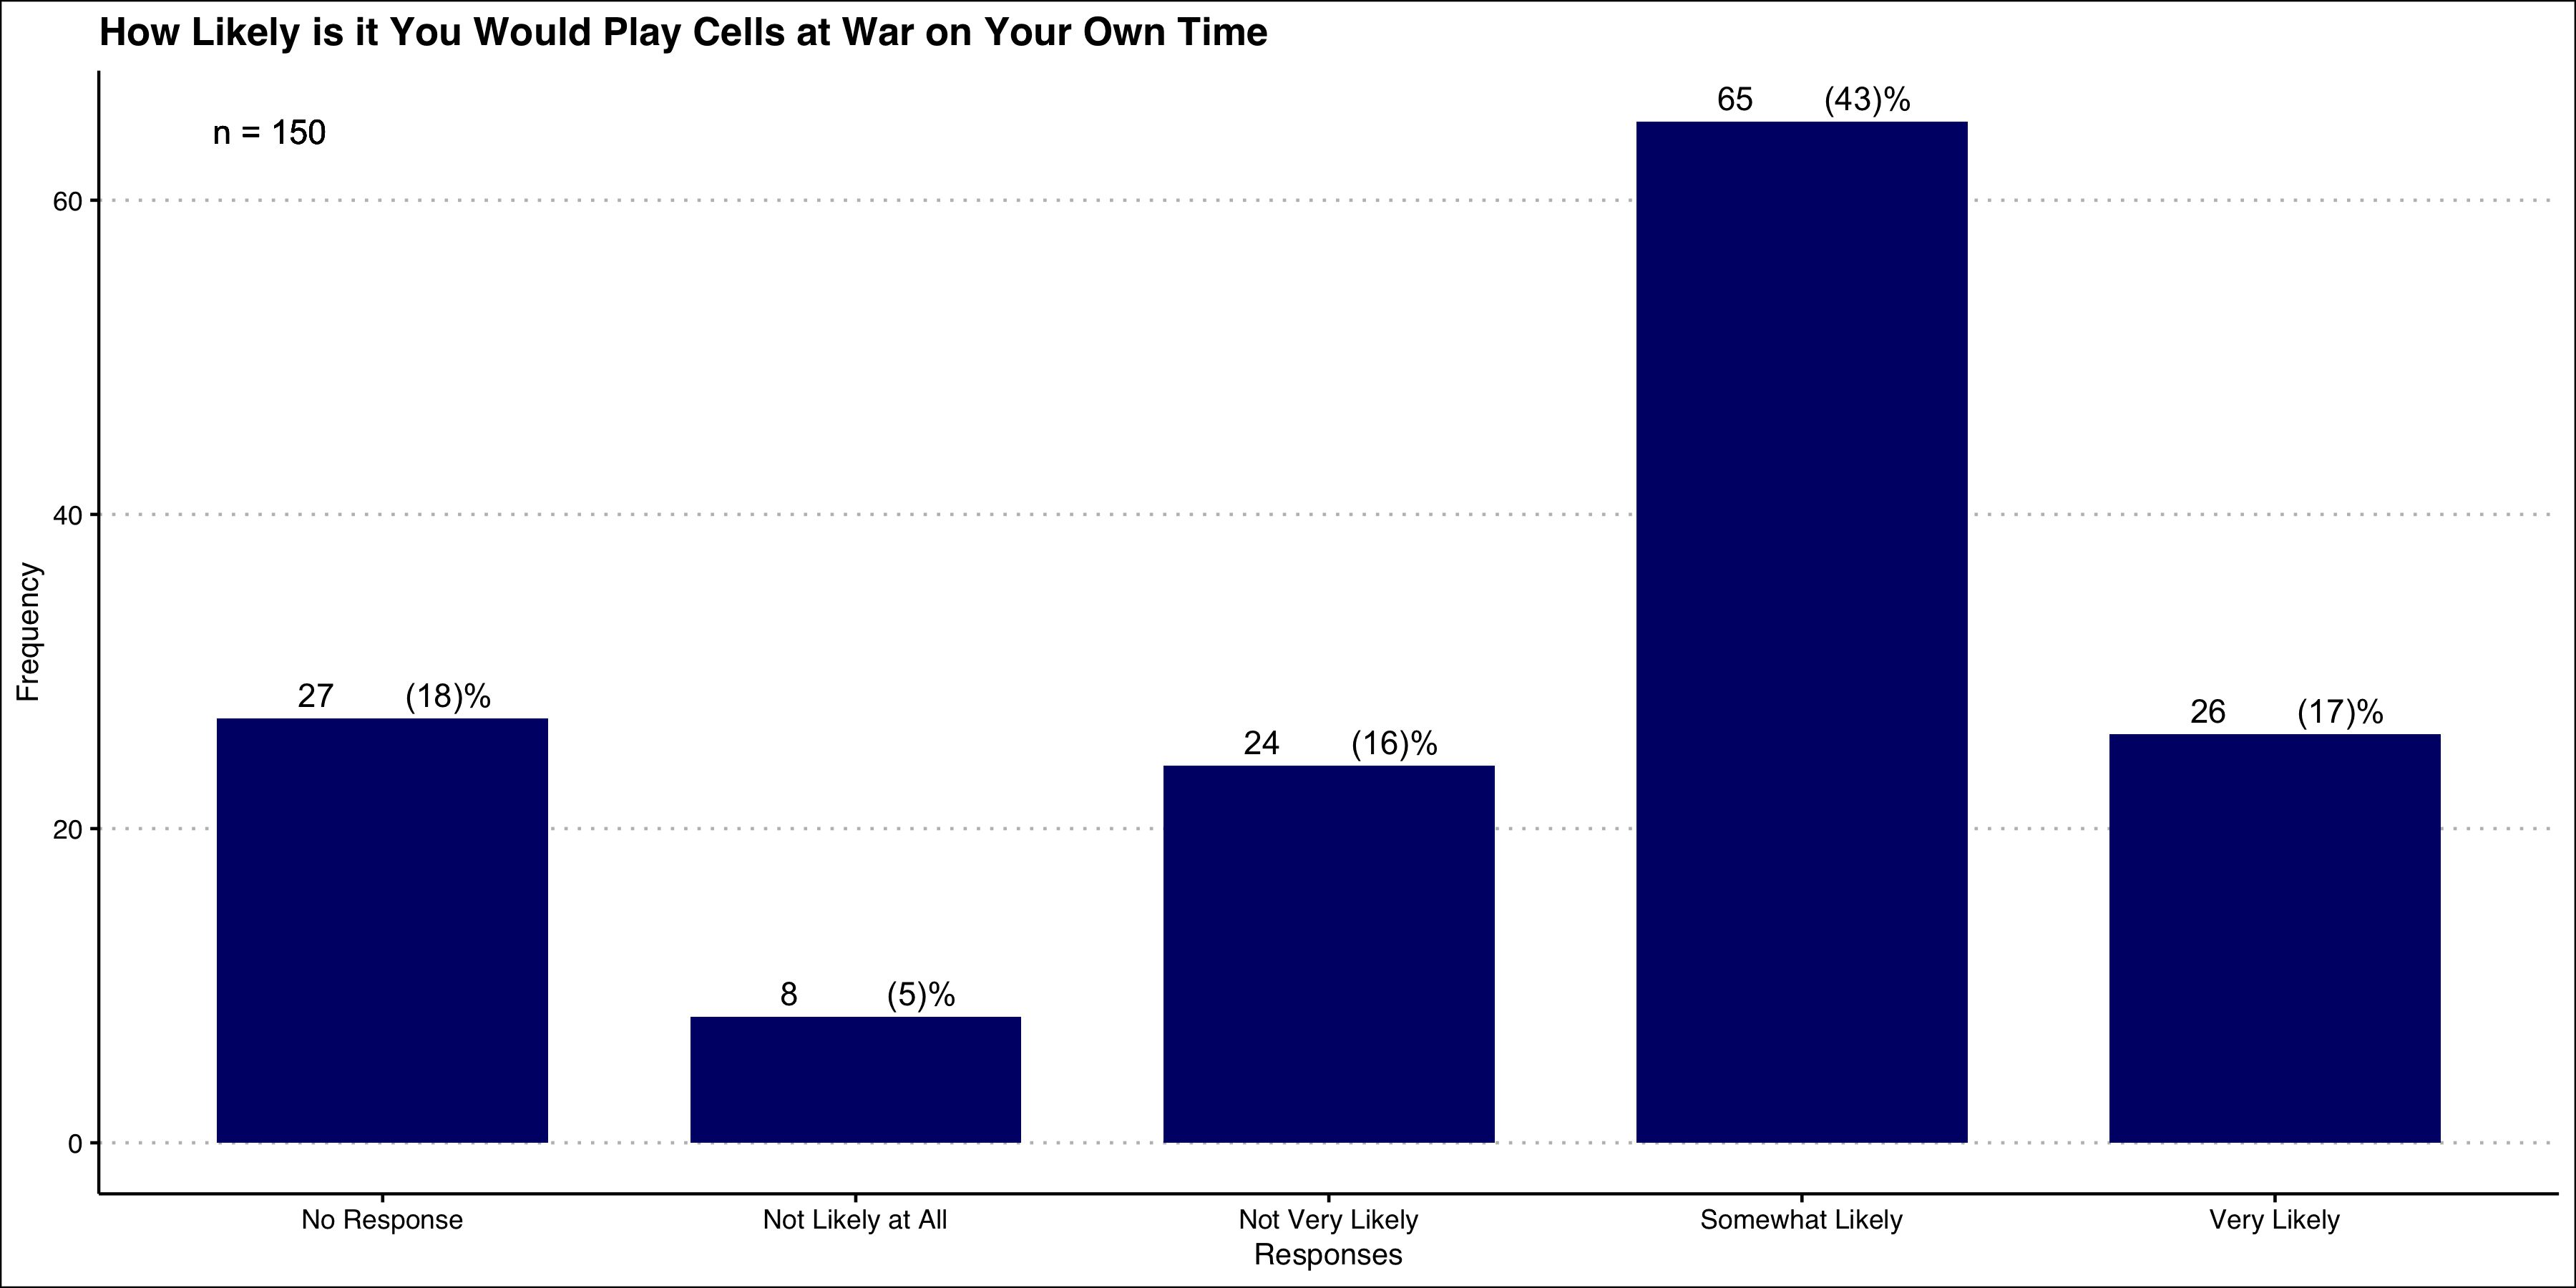
\includegraphics[width=11cm, height=6cm]{how_likely_you_would_play_cellsatwar.jpg}
		\end{center}
	\end{frame}

	\begin{frame}{How Prepared Would you Feel if Given a Quiz on Pompe Disease based on Cells at War, Compared to Studying off Traditional Lecture Slides}
		\begin{center}
			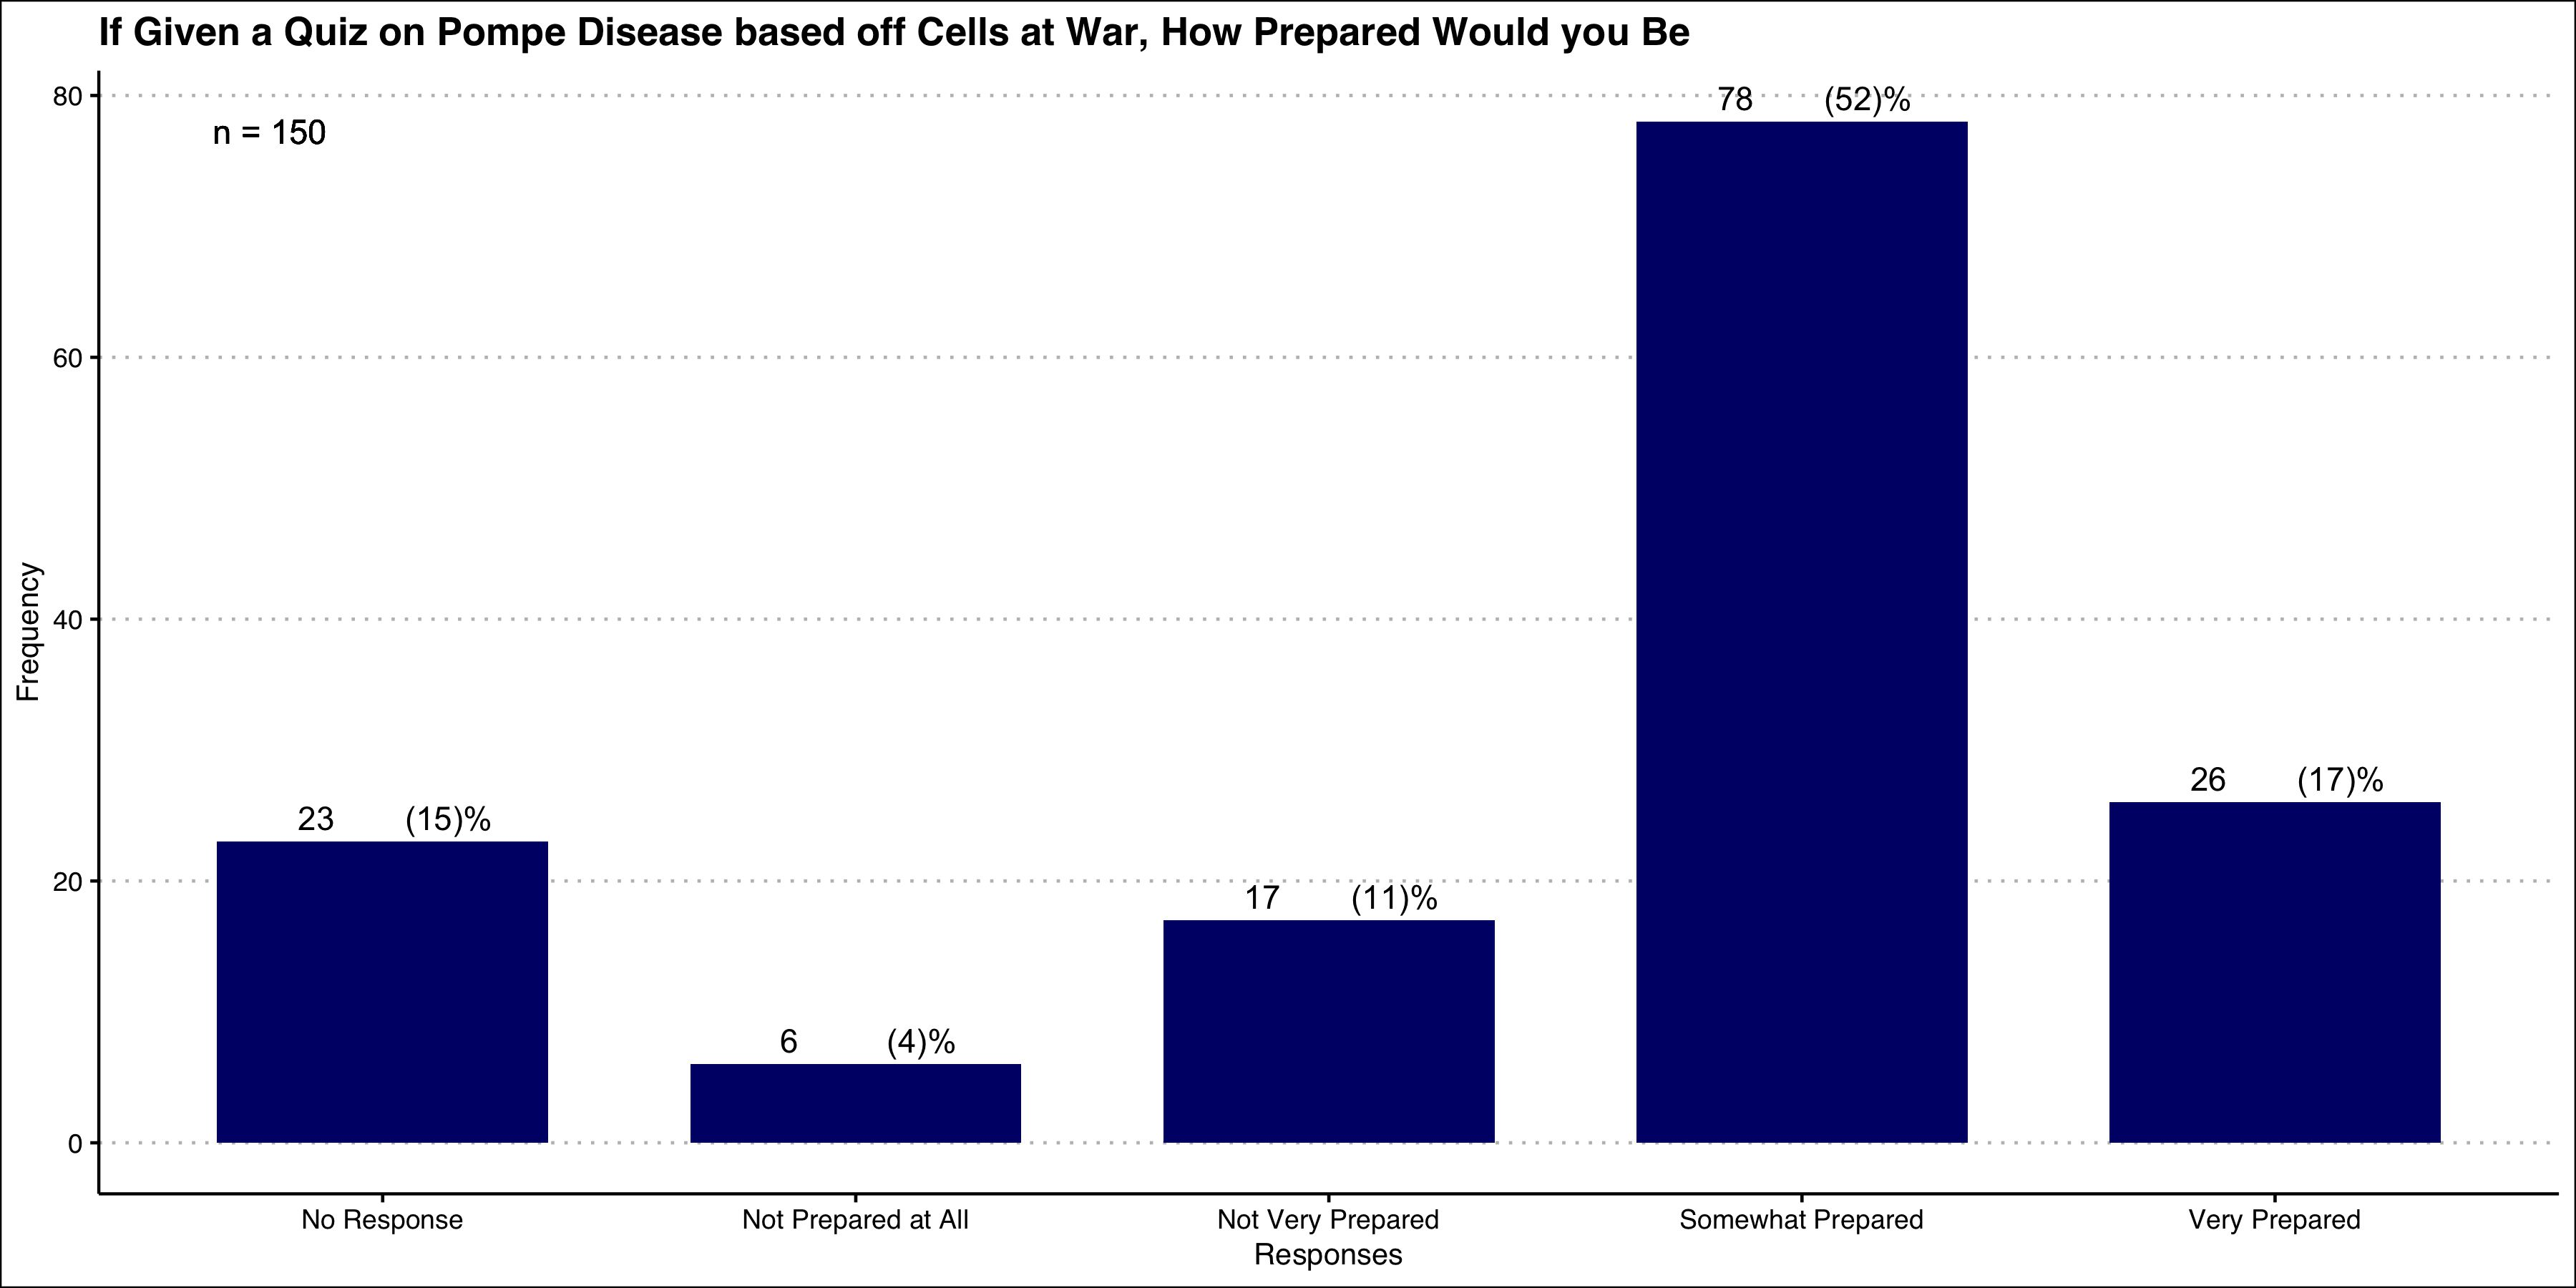
\includegraphics[width=11cm, height=6cm]{how_prepared_if_tested_on_pompe_based_off_cellsatwar.jpg}
		\end{center}
	\end{frame}

	\section{Conclusion}
	\begin{frame}{Conclusions}
		\begin{enumerate}	
			\item Game based learning approaches have the potential to be utilized during lecture as interactive educational tools for students. \newline
			\item Implementing Game-based learning practices could improve student motivation to apply and analyze what they learn, and use it to form new understandings of concepts. \newline
			\item In a cohort where many students did not play video games, learning to play did not distract from understanding the content. \newline
			\item Not only benefits for the students playing the game, but also for the team of students and supervisors from different schools, in different programs, working in collaboration with eachother.
		\end{enumerate}
	\end{frame}

	\section{Future Work}
	\begin{frame}{Future Work}
		\begin{itemize}
			\item Develop games based on different diseases to add to the Cells at War Suite of Games
			\item Expand the use of video games to other domains across STEAM (Physics, Music, Etc...)
			\item International collaboration between more Universities and Colleges	
		\end{itemize}
	\begin{columns}
		\begin{column}{0.4\textwidth}
			\movie[width=5cm,height=3cm,showcontrols=true]{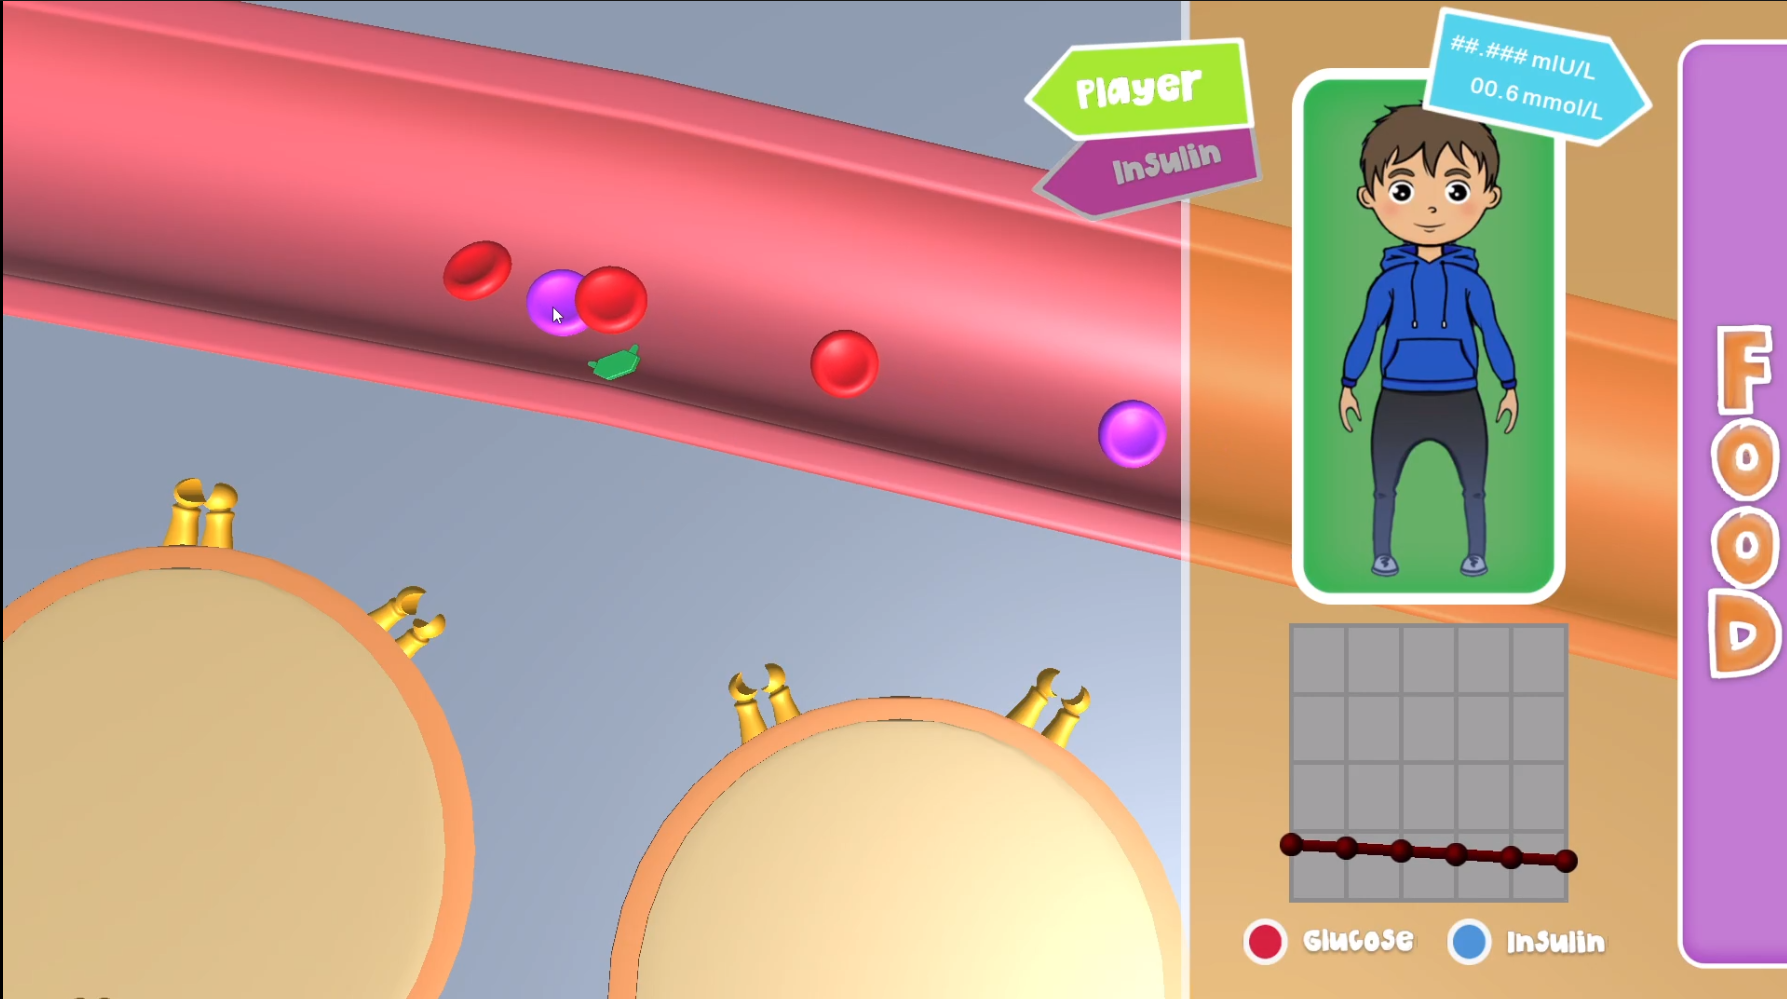
\includegraphics[width=5cm, height=3cm]{tid_thumbnail.png}}{biodemonstration.mp4}
		\end{column}
		\begin{column}{0.3\textwidth}
			
\includegraphics[width=3cm,height=3cm]{wgong.jpeg}
		\end{column}
	\end{columns}	

	\end{frame}
	
	\section{Acknowledgements}
	\begin{frame}{Acknowledgements}
		Thank you...
		\begin{itemize}
			\item Dr. Rosa da Silva (McMaster)
			\item Jean Paul Amore (GBC)
			\item Bianca Flaim
			
		\end{itemize}
	\centering
	
\includegraphics[width=5cm, height=3cm]{gbc.png}	
	
\includegraphics[width=10cm, height=3cm]{cewil.jpg}
	\end{frame}

\end{document}
